% SPDX-FileCopyrightText: 2026 Piotr Gródek and the RadVeil contributors
% SPDX-License-Identifier: CC-BY-SA-4.0
%
% Licence: CC BY-SA 4.0, because Figure 1 and the per-case results derive
% from IXI (CC BY-SA). Every number in this manuscript is a macro from
% generated/numbers.tex or a table body from generated/tab_*.tex, both
% written by ../analysis/make_assets.py from ../results/. Do not type
% numbers in here; see ../README.md.
\documentclass[11pt]{article}
\usepackage[a4paper,margin=2.4cm]{geometry}
\usepackage[T1]{fontenc}
\usepackage[utf8]{inputenc}
\usepackage{lmodern}
\usepackage{graphicx}
\usepackage{booktabs}
\usepackage{amsmath,amssymb}
\usepackage{microtype}
\usepackage{xcolor}
\usepackage[hidelinks]{hyperref}
\usepackage[numbers,sort&compress]{natbib}
\usepackage{caption}
\captionsetup{font=small,labelfont=bf}
\usepackage{tikz}
\usetikzlibrary{arrows.meta,positioning}
% let floats fill pages instead of piling up behind the bibliography
\renewcommand{\topfraction}{0.9}
\renewcommand{\floatpagefraction}{0.8}
\setcounter{topnumber}{3}

\graphicspath{{figures/}}
% generated by paper/analysis/make_assets.py -- do not edit
\newcommand{\atkAdaptiveEarsMediapipeAnyPct}{89}
\newcommand{\atkAdaptiveEarsMediapipeCorePct}{31}
\newcommand{\atkAdaptiveEarsMediapipeN}{110}
\newcommand{\atkAdaptiveEarsYunetAnyPct}{81}
\newcommand{\atkAdaptiveEarsYunetCorePct}{54}
\newcommand{\atkAdaptiveEarsYunetN}{109}
\newcommand{\atkAdaptiveMediapipeAnyPct}{84}
\newcommand{\atkAdaptiveMediapipeCorePct}{39}
\newcommand{\atkAdaptiveMediapipeN}{110}
\newcommand{\atkAdaptiveNoverifyMediapipeAnyPct}{100}
\newcommand{\atkAdaptiveNoverifyMediapipeCorePct}{59}
\newcommand{\atkAdaptiveNoverifyMediapipeN}{110}
\newcommand{\atkAdaptiveNoverifyYunetAnyPct}{98}
\newcommand{\atkAdaptiveNoverifyYunetCorePct}{83}
\newcommand{\atkAdaptiveNoverifyYunetN}{109}
\newcommand{\atkAdaptiveYunetAnyPct}{87}
\newcommand{\atkAdaptiveYunetCorePct}{65}
\newcommand{\atkAdaptiveYunetN}{109}
\newcommand{\atkBlurMediapipeAnyPct}{91}
\newcommand{\atkBlurMediapipeCorePct}{42}
\newcommand{\atkBlurMediapipeN}{110}
\newcommand{\atkBlurYunetAnyPct}{91}
\newcommand{\atkBlurYunetCorePct}{68}
\newcommand{\atkBlurYunetN}{109}
\newcommand{\atkCutMediapipeAnyPct}{36}
\newcommand{\atkCutMediapipeCorePct}{8}
\newcommand{\atkCutMediapipeN}{110}
\newcommand{\atkCutYunetAnyPct}{59}
\newcommand{\atkCutYunetCorePct}{11}
\newcommand{\atkCutYunetN}{109}
\newcommand{\atkMriDefaceMediapipeAnyPct}{99}
\newcommand{\atkMriDefaceMediapipeCorePct}{92}
\newcommand{\atkMriDefaceMediapipeN}{110}
\newcommand{\atkMriDefaceYunetAnyPct}{95}
\newcommand{\atkMriDefaceYunetCorePct}{84}
\newcommand{\atkMriDefaceYunetN}{109}
\newcommand{\atkPairedN}{110}
\newcommand{\atkPydefaceMediapipeAnyPct}{95}
\newcommand{\atkPydefaceMediapipeCorePct}{37}
\newcommand{\atkPydefaceMediapipeN}{110}
\newcommand{\atkPydefaceYunetAnyPct}{99}
\newcommand{\atkPydefaceYunetCorePct}{93}
\newcommand{\atkPydefaceYunetN}{109}
\newcommand{\atkQuickshearMediapipeAnyPct}{98}
\newcommand{\atkQuickshearMediapipeCorePct}{58}
\newcommand{\atkQuickshearMediapipeN}{110}
\newcommand{\atkQuickshearYunetAnyPct}{96}
\newcommand{\atkQuickshearYunetCorePct}{62}
\newcommand{\atkQuickshearYunetN}{109}
\newcommand{\bsAdaptiveAllMedianDist}{6.6}
\newcommand{\bsAdaptiveAllMinDist}{1.3}
\newcommand{\bsAdaptiveAllUpper}{1.5}
\newcommand{\bsAdaptiveAslN}{43}
\newcommand{\bsAdaptiveAslUpper}{7}
\newcommand{\bsAdaptiveEarsAllMedianDist}{4.6}
\newcommand{\bsAdaptiveEarsAllMinDist}{0.0}
\newcommand{\bsAdaptiveEarsAllUpper}{6.4}
\newcommand{\bsAdaptiveEarsLabN}{61}
\newcommand{\bsAdaptiveEarsLabTouched}{0}
\newcommand{\bsAdaptiveEarsMedianDist}{5.0}
\newcommand{\bsAdaptiveEarsMinDist}{0.0}
\newcommand{\bsAdaptiveEarsN}{201}
\newcommand{\bsAdaptiveEarsPairedTouched}{1}
\newcommand{\bsAdaptiveEarsSegMedianDist}{6.1}
\newcommand{\bsAdaptiveEarsTissueMl}{138}
\newcommand{\bsAdaptiveEarsTouched}{7}
\newcommand{\bsAdaptiveEarsUpper}{4.2}
\newcommand{\bsAdaptiveFsmN}{49}
\newcommand{\bsAdaptiveFsmUpper}{6}
\newcommand{\bsAdaptiveGuardAllMedianDist}{6.6}
\newcommand{\bsAdaptiveGuardAllMinDist}{3.6}
\newcommand{\bsAdaptiveGuardAllUpper}{1.5}
\newcommand{\bsAdaptiveGuardLabN}{61}
\newcommand{\bsAdaptiveGuardLabTouched}{0}
\newcommand{\bsAdaptiveGuardMedianDist}{6.4}
\newcommand{\bsAdaptiveGuardMinDist}{3.7}
\newcommand{\bsAdaptiveGuardN}{201}
\newcommand{\bsAdaptiveGuardPairedTouched}{0}
\newcommand{\bsAdaptiveGuardSegMedianDist}{7.3}
\newcommand{\bsAdaptiveGuardTissueMl}{64}
\newcommand{\bsAdaptiveGuardTouched}{0}
\newcommand{\bsAdaptiveGuardUpper}{2.7}
\newcommand{\bsAdaptiveInfantN}{8}
\newcommand{\bsAdaptiveInfantUpper}{31}
\newcommand{\bsAdaptiveIxiN}{91}
\newcommand{\bsAdaptiveIxiUpper}{3}
\newcommand{\bsAdaptiveLabN}{61}
\newcommand{\bsAdaptiveLabTouched}{0}
\newcommand{\bsAdaptiveMedianDist}{6.4}
\newcommand{\bsAdaptiveMinDist}{2.8}
\newcommand{\bsAdaptiveN}{201}
\newcommand{\bsAdaptiveNoverifyAllMedianDist}{6.6}
\newcommand{\bsAdaptiveNoverifyAllMinDist}{1.3}
\newcommand{\bsAdaptiveNoverifyAllUpper}{1.5}
\newcommand{\bsAdaptiveNoverifyLabN}{61}
\newcommand{\bsAdaptiveNoverifyLabTouched}{0}
\newcommand{\bsAdaptiveNoverifyMedianDist}{6.4}
\newcommand{\bsAdaptiveNoverifyMinDist}{2.8}
\newcommand{\bsAdaptiveNoverifyN}{201}
\newcommand{\bsAdaptiveNoverifyPairedTouched}{0}
\newcommand{\bsAdaptiveNoverifySegMedianDist}{7.2}
\newcommand{\bsAdaptiveNoverifyTissueMl}{64}
\newcommand{\bsAdaptiveNoverifyTouched}{0}
\newcommand{\bsAdaptiveNoverifyUpper}{2.7}
\newcommand{\bsAdaptivePairedTouched}{0}
\newcommand{\bsAdaptiveQinN}{10}
\newcommand{\bsAdaptiveQinUpper}{26}
\newcommand{\bsAdaptiveRobustAllMedianDist}{6.3}
\newcommand{\bsAdaptiveRobustAllMinDist}{0.0}
\newcommand{\bsAdaptiveRobustAllUpper}{2.6}
\newcommand{\bsAdaptiveRobustLabN}{61}
\newcommand{\bsAdaptiveRobustLabTouched}{0}
\newcommand{\bsAdaptiveRobustMedianDist}{6.9}
\newcommand{\bsAdaptiveRobustMinDist}{2.8}
\newcommand{\bsAdaptiveRobustN}{356}
\newcommand{\bsAdaptiveRobustPairedTouched}{0}
\newcommand{\bsAdaptiveRobustSegMedianDist}{8.3}
\newcommand{\bsAdaptiveRobustTissueMl}{101}
\newcommand{\bsAdaptiveRobustTouched}{4}
\newcommand{\bsAdaptiveRobustUpper}{2.7}
\newcommand{\bsAdaptiveSegMedianDist}{7.2}
\newcommand{\bsAdaptiveTissueMl}{64}
\newcommand{\bsAdaptiveTouched}{0}
\newcommand{\bsAdaptiveUpper}{2.7}
\newcommand{\bsBlurAllMedianDist}{6.6}
\newcommand{\bsBlurAllMinDist}{1.3}
\newcommand{\bsBlurAllUpper}{1.5}
\newcommand{\bsBlurLabN}{61}
\newcommand{\bsBlurLabTouched}{0}
\newcommand{\bsBlurMedianDist}{6.4}
\newcommand{\bsBlurMinDist}{2.8}
\newcommand{\bsBlurN}{201}
\newcommand{\bsBlurPairedTouched}{0}
\newcommand{\bsBlurSegMedianDist}{7.2}
\newcommand{\bsBlurTissueMl}{64}
\newcommand{\bsBlurTouched}{0}
\newcommand{\bsBlurUpper}{2.7}
\newcommand{\bsCutAllMedianDist}{6.6}
\newcommand{\bsCutAllMinDist}{1.3}
\newcommand{\bsCutAllUpper}{1.5}
\newcommand{\bsCutLabN}{61}
\newcommand{\bsCutLabTouched}{0}
\newcommand{\bsCutMedianDist}{6.4}
\newcommand{\bsCutMinDist}{2.8}
\newcommand{\bsCutN}{201}
\newcommand{\bsCutPairedTouched}{0}
\newcommand{\bsCutSegMedianDist}{7.2}
\newcommand{\bsCutTissueMl}{64}
\newcommand{\bsCutTouched}{0}
\newcommand{\bsCutUpper}{2.7}
\newcommand{\bsMriDefaceAllMedianDist}{3.7}
\newcommand{\bsMriDefaceAllMinDist}{0.0}
\newcommand{\bsMriDefaceAllUpper}{43.6}
\newcommand{\bsMriDefaceLabN}{61}
\newcommand{\bsMriDefaceLabTouched}{1}
\newcommand{\bsMriDefaceMedianDist}{5.7}
\newcommand{\bsMriDefaceMinDist}{0.0}
\newcommand{\bsMriDefaceN}{396}
\newcommand{\bsMriDefacePairedTouched}{31}
\newcommand{\bsMriDefaceSegMedianDist}{7.8}
\newcommand{\bsMriDefaceTissueMl}{396}
\newcommand{\bsMriDefaceTouched}{156}
\newcommand{\bsMriDefaceUpper}{36.1}
\newcommand{\bsPairedN}{110}
\newcommand{\bsPydefaceAllMedianDist}{9.9}
\newcommand{\bsPydefaceAllMinDist}{0.0}
\newcommand{\bsPydefaceAllUpper}{11.5}
\newcommand{\bsPydefaceLabN}{61}
\newcommand{\bsPydefaceLabTouched}{0}
\newcommand{\bsPydefaceMedianDist}{9.9}
\newcommand{\bsPydefaceMinDist}{0.0}
\newcommand{\bsPydefaceN}{111}
\newcommand{\bsPydefacePairedTouched}{6}
\newcommand{\bsPydefaceSegMedianDist}{11.7}
\newcommand{\bsPydefaceTissueMl}{996}
\newcommand{\bsPydefaceTouched}{7}
\newcommand{\bsPydefaceUpper}{10.5}
\newcommand{\bsQuickshearAllMedianDist}{4.7}
\newcommand{\bsQuickshearAllMinDist}{0.0}
\newcommand{\bsQuickshearAllUpper}{1.0}
\newcommand{\bsQuickshearLabN}{61}
\newcommand{\bsQuickshearLabTouched}{0}
\newcommand{\bsQuickshearMedianDist}{4.1}
\newcommand{\bsQuickshearMinDist}{0.0}
\newcommand{\bsQuickshearN}{457}
\newcommand{\bsQuickshearPairedTouched}{1}
\newcommand{\bsQuickshearSegMedianDist}{5.0}
\newcommand{\bsQuickshearTissueMl}{351}
\newcommand{\bsQuickshearTouched}{1}
\newcommand{\bsQuickshearUpper}{4.2}
\newcommand{\deconvArcFaceClean}{86.7}
\newcommand{\deconvArcFacePlain}{0.0}
\newcommand{\deconvArcFaceSigma}{0.0}
\newcommand{\deconvArcFaceSigmaXAdaptive}{0.0}
\newcommand{\deconvIters}{15}
\newcommand{\deconvN}{60}
\newcommand{\deconvSFaceClean}{88.3}
\newcommand{\deconvSFacePlain}{0.0}
\newcommand{\deconvSFaceSigma}{1.7}
\newcommand{\deconvSFaceSigmaXAdaptive}{1.7}
\newcommand{\dsSsAdaptiveDiceMedian}{0.9988}
\newcommand{\dsSsAdaptiveDiceMin}{0.9931}
\newcommand{\dsSsAdaptiveN}{201}
\newcommand{\dsSsAdaptiveVolMax}{0.82}
\newcommand{\dsSsCutDiceMedian}{0.9986}
\newcommand{\dsSsCutDiceMin}{0.9936}
\newcommand{\dsSsCutN}{201}
\newcommand{\dsSsCutVolMax}{0.82}
\newcommand{\dsSsMriDefaceDiceMedian}{0.9970}
\newcommand{\dsSsMriDefaceDiceMin}{0.9498}
\newcommand{\dsSsMriDefaceN}{396}
\newcommand{\dsSsMriDefaceVolMax}{7.50}
\newcommand{\dsSsPydefaceDiceMedian}{0.9951}
\newcommand{\dsSsPydefaceDiceMin}{0.9849}
\newcommand{\dsSsPydefaceN}{104}
\newcommand{\dsSsPydefaceVolMax}{2.22}
\newcommand{\dsSsQuickshearDiceMedian}{0.9956}
\newcommand{\dsSsQuickshearDiceMin}{0.9710}
\newcommand{\dsSsQuickshearN}{457}
\newcommand{\dsSsQuickshearVolMax}{4.38}
\newcommand{\dtypeMriDefaceChanged}{149}
\newcommand{\dtypePydefaceChanged}{0}
\newcommand{\dtypeQuickshearChanged}{0}
\newcommand{\earDetected}{359}
\newcommand{\earDetectedPct}{89.3}
\newcommand{\earRois}{402}
\newcommand{\earScans}{201}
\newcommand{\flIxiAcceptedNoFace}{0}
\newcommand{\flIxiCorrectRefusals}{0}
\newcommand{\flIxiFace}{311}
\newcommand{\flIxiFaceN}{311}
\newcommand{\flIxiFalseRefusalErrors}{0}
\newcommand{\flIxiFalseRefusalInfant}{0}
\newcommand{\flIxiFalseRefusalPct}{0.6}
\newcommand{\flIxiFalseRefusals}{2}
\newcommand{\flIxiLabelled}{1234}
\newcommand{\flIxiNoFaceN}{0}
\newcommand{\flIxiNone}{0}
\newcommand{\flIxiNotOkN}{617}
\newcommand{\flIxiNotOkPartial}{615}
\newcommand{\flIxiPartial}{923}
\newcommand{\flIxiPartialAccepted}{308}
\newcommand{\flIxiPartialN}{923}
\newcommand{\flIxiUnsure}{0}
\newcommand{\flReviewers}{1}
\newcommand{\flSynthstripAcceptedNoFace}{49}
\newcommand{\flSynthstripCorrectRefusals}{165}
\newcommand{\flSynthstripFace}{106}
\newcommand{\flSynthstripFaceN}{106}
\newcommand{\flSynthstripFalseRefusalErrors}{0}
\newcommand{\flSynthstripFalseRefusalInfant}{8}
\newcommand{\flSynthstripFalseRefusalPct}{7.5}
\newcommand{\flSynthstripFalseRefusals}{8}
\newcommand{\flSynthstripLabelled}{582}
\newcommand{\flSynthstripNoFaceN}{214}
\newcommand{\flSynthstripNone}{214}
\newcommand{\flSynthstripNotOkN}{381}
\newcommand{\flSynthstripNotOkPartial}{208}
\newcommand{\flSynthstripPartial}{262}
\newcommand{\flSynthstripPartialAccepted}{54}
\newcommand{\flSynthstripPartialN}{262}
\newcommand{\flSynthstripUnsure}{0}
\newcommand{\fsmAccepted}{49}
\newcommand{\fsmAcceptedNoFace}{1}
\newcommand{\fsmNoFaceMinDist}{5.8}
\newcommand{\hwCores}{14}
\newcommand{\hwCpu}{Apple M4 Pro}
\newcommand{\hwMem}{48.0}
\newcommand{\ixiAccAgeAndOverPct}{66.6}
\newcommand{\ixiAccAgeToPct}{68.3}
\newcommand{\ixiAccAgeUnderPct}{59.4}
\newcommand{\ixiAccAgeUnknownPct}{61.1}
\newcommand{\ixiAccDevelopmentSubjectsPct}{59.7}
\newcommand{\ixiAccHeldOutSubjectsPct}{65.0}
\newcommand{\ixiAccMenPct}{58.7}
\newcommand{\ixiAccPdPct}{46.9}
\newcommand{\ixiAccTOnePct}{99.7}
\newcommand{\ixiAccTTwoPct}{46.7}
\newcommand{\ixiAccWomenPct}{69.3}
\newcommand{\ixiAccepted}{1120}
\newcommand{\ixiAcceptedPct}{64.5}
\newcommand{\ixiAdaptiveEarsAccepted}{1120}
\newcommand{\ixiAdaptiveEarsFailed}{617}
\newcommand{\ixiBitExact}{1120}
\newcommand{\ixiBrainChecked}{1120}
\newcommand{\ixiBrainTouched}{11}
\newcommand{\ixiBrainTouchedUpper}{1.6}
\newcommand{\ixiCutAccepted}{1120}
\newcommand{\ixiCutFailed}{617}
\newcommand{\ixiDevSubjects}{53}
\newcommand{\ixiErrors}{48}
\newcommand{\ixiEscalated}{109}
\newcommand{\ixiMriDefaceAccepted}{221}
\newcommand{\ixiMriDefaceFailed}{77}
\newcommand{\ixiPydefaceAccepted}{0}
\newcommand{\ixiPydefaceFailed}{298}
\newcommand{\ixiQuickshearAccepted}{298}
\newcommand{\ixiQuickshearFailed}{0}
\newcommand{\ixiRefAdaptiveEarsMedianDist}{3.0}
\newcommand{\ixiRefAdaptiveEarsN}{5}
\newcommand{\ixiRefAdaptiveEarsTouched}{0}
\newcommand{\ixiRefAdaptiveEarsUpper}{45.1}
\newcommand{\ixiRefAdaptiveMedianDist}{5.2}
\newcommand{\ixiRefAdaptiveN}{5}
\newcommand{\ixiRefAdaptiveNoverifyMedianDist}{5.2}
\newcommand{\ixiRefAdaptiveNoverifyN}{5}
\newcommand{\ixiRefAdaptiveNoverifyTouched}{0}
\newcommand{\ixiRefAdaptiveNoverifyUpper}{45.1}
\newcommand{\ixiRefAdaptiveTouched}{0}
\newcommand{\ixiRefAdaptiveUpper}{45.1}
\newcommand{\ixiRefCutMedianDist}{5.2}
\newcommand{\ixiRefCutN}{5}
\newcommand{\ixiRefCutTouched}{0}
\newcommand{\ixiRefCutUpper}{45.1}
\newcommand{\ixiRefMriDefaceMedianDist}{0.9}
\newcommand{\ixiRefMriDefaceN}{221}
\newcommand{\ixiRefMriDefaceTouched}{106}
\newcommand{\ixiRefMriDefaceUpper}{53.7}
\newcommand{\ixiRefQuickshearMedianDist}{3.8}
\newcommand{\ixiRefQuickshearN}{298}
\newcommand{\ixiRefQuickshearTouched}{0}
\newcommand{\ixiRefQuickshearUpper}{1.0}
\newcommand{\ixiRefused}{569}
\newcommand{\ixiResidualAccepted}{1}
\newcommand{\ixiSubjects}{582}
\newcommand{\ixiVolumes}{1737}
\newcommand{\noverifyStatusDiffs}{0}
\newcommand{\profCohortMaxS}{2.48}
\newcommand{\profCohortMedianS}{0.70}
\newcommand{\profCohortN}{40}
\newcommand{\profCohortPNinetyS}{1.80}
\newcommand{\profEffortBalancedS}{0.53}
\newcommand{\profEffortFastS}{0.38}
\newcommand{\profEffortThoroughS}{0.86}
\newcommand{\profMaxThreads}{14}
\newcommand{\profMedianBrainCheckS}{3.8}
\newcommand{\profMedianDetectMs}{7.9}
\newcommand{\profMedianPipelineMs}{427}
\newcommand{\profMedianRenderMs}{9.4}
\newcommand{\profMedianVerifyShare}{66}
\newcommand{\profPeakRssMax}{945}
\newcommand{\profPeakRssMedian}{490}
\newcommand{\profSimdSpeedup}{1.03}
\newcommand{\profSpeedupMax}{3.0}
\newcommand{\profStageN}{22}
\newcommand{\profThroughputMax}{3.5}
\newcommand{\profThroughputOne}{1.2}
\newcommand{\profThroughputVolumes}{56}
\newcommand{\qaFlagged}{\textbf{??}}
\newcommand{\qaReviewed}{\textbf{??}}
\newcommand{\qaSheets}{13031}
\newcommand{\refExpertDice}{0.969}
\newcommand{\refusedFaceIxi}{485}
\newcommand{\refusedFaceSynthstrip}{240}
\newcommand{\refusedIxi}{569}
\newcommand{\refusedSynthstrip}{375}
\newcommand{\reidArcFaceAdaptiveAccAuc}{0.74}
\newcommand{\reidArcFaceAdaptiveAccControl}{92.4}
\newcommand{\reidArcFaceAdaptiveAccDepthFour}{7.2}
\newcommand{\reidArcFaceAdaptiveAccDepthFourChance}{0.18}
\newcommand{\reidArcFaceAdaptiveAccDepthFourControl}{41.7}
\newcommand{\reidArcFaceAdaptiveAccDepthOne}{0.2}
\newcommand{\reidArcFaceAdaptiveAccDepthOneChance}{0.17}
\newcommand{\reidArcFaceAdaptiveAccDepthOneControl}{98.1}
\newcommand{\reidArcFaceAdaptiveAccDepthTwo}{5.4}
\newcommand{\reidArcFaceAdaptiveAccDepthTwoChance}{0.17}
\newcommand{\reidArcFaceAdaptiveAccDepthTwoControl}{72.7}
\newcommand{\reidArcFaceAdaptiveAccP}{10^{-49}}
\newcommand{\reidArcFaceAdaptiveAccRank}{7.4}
\newcommand{\reidArcFaceAdaptiveAccRankHi}{9.6}
\newcommand{\reidArcFaceAdaptiveAccRankLo}{5.4}
\newcommand{\reidArcFaceAdaptiveAccTar}{3.0}
\newcommand{\reidArcFaceAdaptiveAccTarAnonCal}{1.2}
\newcommand{\reidArcFaceAdaptiveAccTenRank}{21.0}
\newcommand{\reidArcFaceAdaptiveAccepted}{539}
\newcommand{\reidArcFaceAdaptiveBlindRank}{3.2}
\newcommand{\reidArcFaceAdaptiveControlRankAtEightyFour}{96.6}
\newcommand{\reidArcFaceAdaptiveEarsAccAuc}{0.74}
\newcommand{\reidArcFaceAdaptiveEarsAccControl}{92.4}
\newcommand{\reidArcFaceAdaptiveEarsAccDepthFour}{8.3}
\newcommand{\reidArcFaceAdaptiveEarsAccDepthFourChance}{0.18}
\newcommand{\reidArcFaceAdaptiveEarsAccDepthFourControl}{41.7}
\newcommand{\reidArcFaceAdaptiveEarsAccDepthOne}{0.2}
\newcommand{\reidArcFaceAdaptiveEarsAccDepthOneChance}{0.17}
\newcommand{\reidArcFaceAdaptiveEarsAccDepthOneControl}{98.1}
\newcommand{\reidArcFaceAdaptiveEarsAccDepthTwo}{5.0}
\newcommand{\reidArcFaceAdaptiveEarsAccDepthTwoChance}{0.17}
\newcommand{\reidArcFaceAdaptiveEarsAccDepthTwoControl}{72.7}
\newcommand{\reidArcFaceAdaptiveEarsAccP}{4.1\times10^{-53}}
\newcommand{\reidArcFaceAdaptiveEarsAccRank}{8.0}
\newcommand{\reidArcFaceAdaptiveEarsAccRankHi}{10.4}
\newcommand{\reidArcFaceAdaptiveEarsAccRankLo}{5.9}
\newcommand{\reidArcFaceAdaptiveEarsAccTar}{3.2}
\newcommand{\reidArcFaceAdaptiveEarsAccTarAnonCal}{1.4}
\newcommand{\reidArcFaceAdaptiveEarsAccTenRank}{22.1}
\newcommand{\reidArcFaceAdaptiveEarsAccepted}{539}
\newcommand{\reidArcFaceAdaptiveEarsBlindRank}{4.6}
\newcommand{\reidArcFaceAdaptiveEarsControlRankAtEightyFour}{96.6}
\newcommand{\reidArcFaceAdaptiveEarsMatchedRank}{3.5}
\newcommand{\reidArcFaceAdaptiveEarsRankAtEightyFour}{17.3}
\newcommand{\reidArcFaceAdaptiveEarsRisk}{46.0}
\newcommand{\reidArcFaceAdaptiveEarsRiskHi}{49.6}
\newcommand{\reidArcFaceAdaptiveEarsRiskLo}{42.5}
\newcommand{\reidArcFaceAdaptiveEarsSameRank}{52.8}
\newcommand{\reidArcFaceAdaptiveMatchedRank}{4.8}
\newcommand{\reidArcFaceAdaptiveNoverifyAccAuc}{0.75}
\newcommand{\reidArcFaceAdaptiveNoverifyAccControl}{92.4}
\newcommand{\reidArcFaceAdaptiveNoverifyAccDepthFour}{7.2}
\newcommand{\reidArcFaceAdaptiveNoverifyAccDepthFourChance}{0.18}
\newcommand{\reidArcFaceAdaptiveNoverifyAccDepthFourControl}{41.7}
\newcommand{\reidArcFaceAdaptiveNoverifyAccDepthOne}{0.4}
\newcommand{\reidArcFaceAdaptiveNoverifyAccDepthOneChance}{0.17}
\newcommand{\reidArcFaceAdaptiveNoverifyAccDepthOneControl}{98.1}
\newcommand{\reidArcFaceAdaptiveNoverifyAccDepthTwo}{5.2}
\newcommand{\reidArcFaceAdaptiveNoverifyAccDepthTwoChance}{0.17}
\newcommand{\reidArcFaceAdaptiveNoverifyAccDepthTwoControl}{72.7}
\newcommand{\reidArcFaceAdaptiveNoverifyAccP}{4.8\times10^{-48}}
\newcommand{\reidArcFaceAdaptiveNoverifyAccRank}{7.2}
\newcommand{\reidArcFaceAdaptiveNoverifyAccRankHi}{9.5}
\newcommand{\reidArcFaceAdaptiveNoverifyAccRankLo}{5.1}
\newcommand{\reidArcFaceAdaptiveNoverifyAccTar}{3.0}
\newcommand{\reidArcFaceAdaptiveNoverifyAccTarAnonCal}{1.2}
\newcommand{\reidArcFaceAdaptiveNoverifyAccTenRank}{21.2}
\newcommand{\reidArcFaceAdaptiveNoverifyAccepted}{539}
\newcommand{\reidArcFaceAdaptiveNoverifyBlindRank}{3.2}
\newcommand{\reidArcFaceAdaptiveNoverifyControlRankAtEightyFour}{96.6}
\newcommand{\reidArcFaceAdaptiveNoverifyMatchedRank}{7.4}
\newcommand{\reidArcFaceAdaptiveNoverifyRankAtEightyFour}{16.0}
\newcommand{\reidArcFaceAdaptiveNoverifyRisk}{45.6}
\newcommand{\reidArcFaceAdaptiveNoverifyRiskHi}{49.1}
\newcommand{\reidArcFaceAdaptiveNoverifyRiskLo}{42.0}
\newcommand{\reidArcFaceAdaptiveNoverifySameRank}{59.0}
\newcommand{\reidArcFaceAdaptiveRankAtEightyFour}{15.8}
\newcommand{\reidArcFaceAdaptiveRisk}{45.7}
\newcommand{\reidArcFaceAdaptiveRiskHi}{49.5}
\newcommand{\reidArcFaceAdaptiveRiskLo}{42.3}
\newcommand{\reidArcFaceAdaptiveSameRank}{53.8}
\newcommand{\reidArcFaceChance}{0.17}
\newcommand{\reidArcFaceControlAuc}{0.99}
\newcommand{\reidArcFaceControlRankFused}{88.6}
\newcommand{\reidArcFaceControlRankOne}{95.0}
\newcommand{\reidArcFaceControlTar}{75.4}
\newcommand{\reidArcFaceCutAccAuc}{0.55}
\newcommand{\reidArcFaceCutAccControl}{92.4}
\newcommand{\reidArcFaceCutAccDepthFour}{0.7}
\newcommand{\reidArcFaceCutAccDepthFourChance}{0.18}
\newcommand{\reidArcFaceCutAccDepthFourControl}{41.7}
\newcommand{\reidArcFaceCutAccDepthOne}{1.5}
\newcommand{\reidArcFaceCutAccDepthOneChance}{0.17}
\newcommand{\reidArcFaceCutAccDepthOneControl}{98.1}
\newcommand{\reidArcFaceCutAccDepthTwo}{1.3}
\newcommand{\reidArcFaceCutAccDepthTwoChance}{0.17}
\newcommand{\reidArcFaceCutAccDepthTwoControl}{72.7}
\newcommand{\reidArcFaceCutAccP}{0.015}
\newcommand{\reidArcFaceCutAccRank}{0.7}
\newcommand{\reidArcFaceCutAccRankHi}{3.3}
\newcommand{\reidArcFaceCutAccRankLo}{0.4}
\newcommand{\reidArcFaceCutAccTar}{0.4}
\newcommand{\reidArcFaceCutAccTarAnonCal}{0.8}
\newcommand{\reidArcFaceCutAccTenRank}{3.0}
\newcommand{\reidArcFaceCutAccepted}{539}
\newcommand{\reidArcFaceCutBlindRank}{0.6}
\newcommand{\reidArcFaceCutControlRankAtEightyFour}{96.6}
\newcommand{\reidArcFaceCutMatchedRank}{1.1}
\newcommand{\reidArcFaceCutRankAtEightyFour}{2.4}
\newcommand{\reidArcFaceCutRisk}{42.3}
\newcommand{\reidArcFaceCutRiskHi}{46.1}
\newcommand{\reidArcFaceCutRiskLo}{38.7}
\newcommand{\reidArcFaceCutSameRank}{0.9}
\newcommand{\reidArcFaceExcluded}{86}
\newcommand{\reidArcFaceGallery}{580}
\newcommand{\reidArcFaceGalleryFour}{571}
\newcommand{\reidArcFacePairedAdaptiveEarsRank}{50.6}
\newcommand{\reidArcFacePairedAdaptiveNoverifyRank}{50.0}
\newcommand{\reidArcFacePairedAdaptiveRank}{49.4}
\newcommand{\reidArcFacePairedControlRank}{87.8}
\newcommand{\reidArcFacePairedCutRank}{45.6}
\newcommand{\reidArcFacePairedMriDefaceRank}{\textbf{??}}
\newcommand{\reidArcFacePairedProbes}{180}
\newcommand{\reidArcFacePairedPydefaceRank}{\textbf{??}}
\newcommand{\reidArcFacePairedQuickshearRank}{85.0}
\newcommand{\reidArcFacePairedSubjects}{93}
\newcommand{\reidArcFaceProbeScans}{1066}
\newcommand{\reidArcFaceQuickshearAccAuc}{0.75}
\newcommand{\reidArcFaceQuickshearAccControl}{71.4}
\newcommand{\reidArcFaceQuickshearAccDepthFour}{0.0}
\newcommand{\reidArcFaceQuickshearAccDepthFourChance}{0.18}
\newcommand{\reidArcFaceQuickshearAccDepthFourControl}{20.0}
\newcommand{\reidArcFaceQuickshearAccDepthOne}{14.3}
\newcommand{\reidArcFaceQuickshearAccDepthOneChance}{0.17}
\newcommand{\reidArcFaceQuickshearAccDepthOneControl}{85.7}
\newcommand{\reidArcFaceQuickshearAccDepthTwo}{14.3}
\newcommand{\reidArcFaceQuickshearAccDepthTwoChance}{0.17}
\newcommand{\reidArcFaceQuickshearAccDepthTwoControl}{57.1}
\newcommand{\reidArcFaceQuickshearAccP}{1.000}
\newcommand{\reidArcFaceQuickshearAccRank}{0.0}
\newcommand{\reidArcFaceQuickshearAccRankHi}{60.2}
\newcommand{\reidArcFaceQuickshearAccRankLo}{0.0}
\newcommand{\reidArcFaceQuickshearAccTar}{56.8}
\newcommand{\reidArcFaceQuickshearAccTarAnonCal}{31.1}
\newcommand{\reidArcFaceQuickshearAccTenRank}{14.3}
\newcommand{\reidArcFaceQuickshearAccepted}{7}
\newcommand{\reidArcFaceQuickshearBlindRank}{0.0}
\newcommand{\reidArcFaceQuickshearControlRankAtEightyFour}{82.6}
\newcommand{\reidArcFaceQuickshearRankAtEightyFour}{12.9}
\newcommand{\reidArcFaceQuickshearRisk}{85.0}
\newcommand{\reidArcFaceQuickshearRiskHi}{90.7}
\newcommand{\reidArcFaceQuickshearRiskLo}{79.0}
\newcommand{\reidArcFaceQuickshearSameRank}{20.0}
\newcommand{\reidSFaceAdaptiveAccAuc}{0.73}
\newcommand{\reidSFaceAdaptiveAccControl}{89.4}
\newcommand{\reidSFaceAdaptiveAccDepthFour}{5.6}
\newcommand{\reidSFaceAdaptiveAccDepthFourChance}{0.18}
\newcommand{\reidSFaceAdaptiveAccDepthFourControl}{27.1}
\newcommand{\reidSFaceAdaptiveAccDepthOne}{0.6}
\newcommand{\reidSFaceAdaptiveAccDepthOneChance}{0.17}
\newcommand{\reidSFaceAdaptiveAccDepthOneControl}{89.8}
\newcommand{\reidSFaceAdaptiveAccDepthTwo}{5.0}
\newcommand{\reidSFaceAdaptiveAccDepthTwoChance}{0.17}
\newcommand{\reidSFaceAdaptiveAccDepthTwoControl}{63.1}
\newcommand{\reidSFaceAdaptiveAccP}{7.6\times10^{-40}}
\newcommand{\reidSFaceAdaptiveAccRank}{6.5}
\newcommand{\reidSFaceAdaptiveAccRankHi}{8.7}
\newcommand{\reidSFaceAdaptiveAccRankLo}{4.4}
\newcommand{\reidSFaceAdaptiveAccTar}{2.9}
\newcommand{\reidSFaceAdaptiveAccTarAnonCal}{3.8}
\newcommand{\reidSFaceAdaptiveAccTenRank}{21.0}
\newcommand{\reidSFaceAdaptiveAccepted}{539}
\newcommand{\reidSFaceAdaptiveBlindRank}{1.9}
\newcommand{\reidSFaceAdaptiveControlRankAtEightyFour}{95.5}
\newcommand{\reidSFaceAdaptiveEarsAccAuc}{0.73}
\newcommand{\reidSFaceAdaptiveEarsAccControl}{89.4}
\newcommand{\reidSFaceAdaptiveEarsAccDepthFour}{6.9}
\newcommand{\reidSFaceAdaptiveEarsAccDepthFourChance}{0.18}
\newcommand{\reidSFaceAdaptiveEarsAccDepthFourControl}{27.1}
\newcommand{\reidSFaceAdaptiveEarsAccDepthOne}{0.6}
\newcommand{\reidSFaceAdaptiveEarsAccDepthOneChance}{0.17}
\newcommand{\reidSFaceAdaptiveEarsAccDepthOneControl}{89.8}
\newcommand{\reidSFaceAdaptiveEarsAccDepthTwo}{5.2}
\newcommand{\reidSFaceAdaptiveEarsAccDepthTwoChance}{0.17}
\newcommand{\reidSFaceAdaptiveEarsAccDepthTwoControl}{63.1}
\newcommand{\reidSFaceAdaptiveEarsAccP}{2.1\times10^{-51}}
\newcommand{\reidSFaceAdaptiveEarsAccRank}{7.6}
\newcommand{\reidSFaceAdaptiveEarsAccRankHi}{9.8}
\newcommand{\reidSFaceAdaptiveEarsAccRankLo}{5.4}
\newcommand{\reidSFaceAdaptiveEarsAccTar}{3.0}
\newcommand{\reidSFaceAdaptiveEarsAccTarAnonCal}{3.6}
\newcommand{\reidSFaceAdaptiveEarsAccTenRank}{20.6}
\newcommand{\reidSFaceAdaptiveEarsAccepted}{539}
\newcommand{\reidSFaceAdaptiveEarsBlindRank}{3.3}
\newcommand{\reidSFaceAdaptiveEarsControlRankAtEightyFour}{95.6}
\newcommand{\reidSFaceAdaptiveEarsMatchedRank}{3.0}
\newcommand{\reidSFaceAdaptiveEarsRankAtEightyFour}{16.1}
\newcommand{\reidSFaceAdaptiveEarsRisk}{39.2}
\newcommand{\reidSFaceAdaptiveEarsRiskHi}{42.7}
\newcommand{\reidSFaceAdaptiveEarsRiskLo}{35.7}
\newcommand{\reidSFaceAdaptiveEarsSameRank}{51.7}
\newcommand{\reidSFaceAdaptiveMatchedRank}{3.2}
\newcommand{\reidSFaceAdaptiveNoverifyAccAuc}{0.74}
\newcommand{\reidSFaceAdaptiveNoverifyAccControl}{89.4}
\newcommand{\reidSFaceAdaptiveNoverifyAccDepthFour}{5.0}
\newcommand{\reidSFaceAdaptiveNoverifyAccDepthFourChance}{0.18}
\newcommand{\reidSFaceAdaptiveNoverifyAccDepthFourControl}{27.1}
\newcommand{\reidSFaceAdaptiveNoverifyAccDepthOne}{0.7}
\newcommand{\reidSFaceAdaptiveNoverifyAccDepthOneChance}{0.17}
\newcommand{\reidSFaceAdaptiveNoverifyAccDepthOneControl}{89.8}
\newcommand{\reidSFaceAdaptiveNoverifyAccDepthTwo}{4.8}
\newcommand{\reidSFaceAdaptiveNoverifyAccDepthTwoChance}{0.17}
\newcommand{\reidSFaceAdaptiveNoverifyAccDepthTwoControl}{63.1}
\newcommand{\reidSFaceAdaptiveNoverifyAccP}{5.2\times10^{-32}}
\newcommand{\reidSFaceAdaptiveNoverifyAccRank}{5.6}
\newcommand{\reidSFaceAdaptiveNoverifyAccRankHi}{7.7}
\newcommand{\reidSFaceAdaptiveNoverifyAccRankLo}{3.5}
\newcommand{\reidSFaceAdaptiveNoverifyAccTar}{3.1}
\newcommand{\reidSFaceAdaptiveNoverifyAccTarAnonCal}{3.8}
\newcommand{\reidSFaceAdaptiveNoverifyAccTenRank}{20.6}
\newcommand{\reidSFaceAdaptiveNoverifyAccepted}{539}
\newcommand{\reidSFaceAdaptiveNoverifyBlindRank}{1.9}
\newcommand{\reidSFaceAdaptiveNoverifyControlRankAtEightyFour}{95.5}
\newcommand{\reidSFaceAdaptiveNoverifyMatchedRank}{10.0}
\newcommand{\reidSFaceAdaptiveNoverifyRankAtEightyFour}{15.5}
\newcommand{\reidSFaceAdaptiveNoverifyRisk}{38.2}
\newcommand{\reidSFaceAdaptiveNoverifyRiskHi}{41.7}
\newcommand{\reidSFaceAdaptiveNoverifyRiskLo}{34.7}
\newcommand{\reidSFaceAdaptiveNoverifySameRank}{60.6}
\newcommand{\reidSFaceAdaptiveRankAtEightyFour}{15.7}
\newcommand{\reidSFaceAdaptiveRisk}{38.6}
\newcommand{\reidSFaceAdaptiveRiskHi}{42.0}
\newcommand{\reidSFaceAdaptiveRiskLo}{35.3}
\newcommand{\reidSFaceAdaptiveSameRank}{50.5}
\newcommand{\reidSFaceChance}{0.17}
\newcommand{\reidSFaceControlAuc}{0.97}
\newcommand{\reidSFaceControlRankFused}{80.6}
\newcommand{\reidSFaceControlRankOne}{79.3}
\newcommand{\reidSFaceControlTar}{69.8}
\newcommand{\reidSFaceCutAccAuc}{0.58}
\newcommand{\reidSFaceCutAccControl}{89.4}
\newcommand{\reidSFaceCutAccDepthFour}{0.6}
\newcommand{\reidSFaceCutAccDepthFourChance}{0.18}
\newcommand{\reidSFaceCutAccDepthFourControl}{27.1}
\newcommand{\reidSFaceCutAccDepthOne}{1.7}
\newcommand{\reidSFaceCutAccDepthOneChance}{0.17}
\newcommand{\reidSFaceCutAccDepthOneControl}{89.8}
\newcommand{\reidSFaceCutAccDepthTwo}{0.7}
\newcommand{\reidSFaceCutAccDepthTwoChance}{0.17}
\newcommand{\reidSFaceCutAccDepthTwoControl}{63.1}
\newcommand{\reidSFaceCutAccP}{5.6\times10^{-6}}
\newcommand{\reidSFaceCutAccRank}{1.9}
\newcommand{\reidSFaceCutAccRankHi}{3.3}
\newcommand{\reidSFaceCutAccRankLo}{0.6}
\newcommand{\reidSFaceCutAccTar}{0.6}
\newcommand{\reidSFaceCutAccTarAnonCal}{0.9}
\newcommand{\reidSFaceCutAccTenRank}{3.9}
\newcommand{\reidSFaceCutAccepted}{539}
\newcommand{\reidSFaceCutBlindRank}{0.7}
\newcommand{\reidSFaceCutControlRankAtEightyFour}{95.6}
\newcommand{\reidSFaceCutMatchedRank}{1.3}
\newcommand{\reidSFaceCutRankAtEightyFour}{3.2}
\newcommand{\reidSFaceCutRisk}{36.3}
\newcommand{\reidSFaceCutRiskHi}{39.8}
\newcommand{\reidSFaceCutRiskLo}{32.7}
\newcommand{\reidSFaceCutSameRank}{2.4}
\newcommand{\reidSFaceExcluded}{86}
\newcommand{\reidSFaceGallery}{580}
\newcommand{\reidSFaceGalleryFour}{571}
\newcommand{\reidSFacePairedAdaptiveEarsRank}{41.1}
\newcommand{\reidSFacePairedAdaptiveNoverifyRank}{40.6}
\newcommand{\reidSFacePairedAdaptiveRank}{40.6}
\newcommand{\reidSFacePairedControlRank}{82.8}
\newcommand{\reidSFacePairedCutRank}{39.4}
\newcommand{\reidSFacePairedProbes}{180}
\newcommand{\reidSFacePairedQuickshearRank}{80.0}
\newcommand{\reidSFacePairedSubjects}{93}
\newcommand{\reidSFaceProbeScans}{1066}
\newcommand{\reidSFaceQuickshearAccAuc}{0.78}
\newcommand{\reidSFaceQuickshearAccControl}{85.7}
\newcommand{\reidSFaceQuickshearAccDepthFour}{20.0}
\newcommand{\reidSFaceQuickshearAccDepthFourChance}{0.18}
\newcommand{\reidSFaceQuickshearAccDepthFourControl}{20.0}
\newcommand{\reidSFaceQuickshearAccDepthOne}{14.3}
\newcommand{\reidSFaceQuickshearAccDepthOneChance}{0.17}
\newcommand{\reidSFaceQuickshearAccDepthOneControl}{71.4}
\newcommand{\reidSFaceQuickshearAccDepthTwo}{0.0}
\newcommand{\reidSFaceQuickshearAccDepthTwoChance}{0.17}
\newcommand{\reidSFaceQuickshearAccDepthTwoControl}{57.1}
\newcommand{\reidSFaceQuickshearAccP}{0.012}
\newcommand{\reidSFaceQuickshearAccRank}{14.3}
\newcommand{\reidSFaceQuickshearAccRankHi}{80.6}
\newcommand{\reidSFaceQuickshearAccRankLo}{0.6}
\newcommand{\reidSFaceQuickshearAccTar}{46.7}
\newcommand{\reidSFaceQuickshearAccTarAnonCal}{40.5}
\newcommand{\reidSFaceQuickshearAccTenRank}{28.6}
\newcommand{\reidSFaceQuickshearAccepted}{7}
\newcommand{\reidSFaceQuickshearBlindRank}{0.0}
\newcommand{\reidSFaceQuickshearControlRankAtEightyFour}{85.7}
\newcommand{\reidSFaceQuickshearRankAtEightyFour}{29.8}
\newcommand{\reidSFaceQuickshearRisk}{80.0}
\newcommand{\reidSFaceQuickshearRiskHi}{86.0}
\newcommand{\reidSFaceQuickshearRiskLo}{73.7}
\newcommand{\reidSFaceQuickshearSameRank}{80.0}
\newcommand{\requantMriDefaceMedian}{0}
\newcommand{\requantMriDefaceN}{396}
\newcommand{\requantMriDefaceScans}{155}
\newcommand{\requantPydefaceMedian}{39114}
\newcommand{\requantPydefaceN}{111}
\newcommand{\requantPydefaceScans}{74}
\newcommand{\requantQuickshearMedian}{0}
\newcommand{\requantQuickshearN}{457}
\newcommand{\requantQuickshearScans}{173}
\newcommand{\retriedCases}{743}
\newcommand{\robustAccepted}{356}
\newcommand{\robustGained}{155}
\newcommand{\robustGainedTouched}{4}
\newcommand{\rustDiceMedian}{0.9964}
\newcommand{\rustDiceMin}{0.9718}
\newcommand{\rustExpertDice}{0.969}
\newcommand{\rustN}{582}
\newcommand{\segAdaptiveClassDiceOne}{0.996}
\newcommand{\segAdaptiveClassDiceThree}{0.999}
\newcommand{\segAdaptiveClassDiceTwo}{0.999}
\newcommand{\segAdaptiveN}{40}
\newcommand{\segCutClassDiceOne}{0.995}
\newcommand{\segCutClassDiceThree}{1.000}
\newcommand{\segCutClassDiceTwo}{0.999}
\newcommand{\segCutN}{40}
\newcommand{\segMriDefaceClassDiceOne}{0.987}
\newcommand{\segMriDefaceClassDiceThree}{0.999}
\newcommand{\segMriDefaceClassDiceTwo}{0.998}
\newcommand{\segMriDefaceN}{76}
\newcommand{\segPydefaceClassDiceOne}{0.981}
\newcommand{\segPydefaceClassDiceThree}{0.996}
\newcommand{\segPydefaceClassDiceTwo}{0.997}
\newcommand{\segPydefaceN}{24}
\newcommand{\segQuickshearClassDiceOne}{0.983}
\newcommand{\segQuickshearClassDiceThree}{0.998}
\newcommand{\segQuickshearClassDiceTwo}{0.998}
\newcommand{\segQuickshearN}{92}
\newcommand{\shapeAdaptiveDeepRank}{22.6}
\newcommand{\shapeAdaptiveEarsOutsideRank}{22.7}
\newcommand{\shapeAdaptiveEarsOutsideRiskRank}{23.5}
\newcommand{\shapeAdaptiveEarsWholeRank}{34.2}
\newcommand{\shapeAdaptiveEarsWholeRiskRank}{36.8}
\newcommand{\shapeAdaptiveNoverifyOutsideRank}{28.3}
\newcommand{\shapeAdaptiveNoverifyOutsideRiskRank}{26.1}
\newcommand{\shapeAdaptiveNoverifyWholeRank}{37.9}
\newcommand{\shapeAdaptiveNoverifyWholeRiskRank}{38.6}
\newcommand{\shapeAdaptiveOutsideRank}{27.5}
\newcommand{\shapeAdaptiveOutsideRiskRank}{25.7}
\newcommand{\shapeAdaptivePoseRank}{18.8}
\newcommand{\shapeAdaptiveWholeRank}{37.2}
\newcommand{\shapeAdaptiveWholeRiskRank}{38.2}
\newcommand{\shapeChance}{0.17}
\newcommand{\shapeControlDeepRank}{22.7}
\newcommand{\shapeControlOutsideRank}{26.0}
\newcommand{\shapeControlPoseRank}{18.7}
\newcommand{\shapeControlPoseSameRank}{21.7}
\newcommand{\shapeControlWholeRank}{41.7}
\newcommand{\shapeCutOutsideRank}{25.1}
\newcommand{\shapeCutOutsideRiskRank}{24.6}
\newcommand{\shapeCutWholeRank}{32.9}
\newcommand{\shapeCutWholeRiskRank}{36.2}
\newcommand{\shapeGallery}{581}
\newcommand{\shapePairedAdaptiveEarsRank}{37.9}
\newcommand{\shapePairedAdaptiveNoverifyRank}{41.9}
\newcommand{\shapePairedAdaptiveRank}{40.4}
\newcommand{\shapePairedControlRank}{46.5}
\newcommand{\shapePairedCutRank}{35.9}
\newcommand{\shapePairedMriDefaceRank}{\textbf{??}}
\newcommand{\shapePairedPydefaceRank}{\textbf{??}}
\newcommand{\shapePairedQuickshearRank}{46.0}
\newcommand{\shapeQuickshearOutsideRank}{30.0}
\newcommand{\shapeQuickshearOutsideRiskRank}{30.3}
\newcommand{\shapeQuickshearWholeRank}{30.0}
\newcommand{\shapeQuickshearWholeRiskRank}{46.0}
\newcommand{\ssAccepted}{201}
\newcommand{\ssBitExact}{201}
\newcommand{\ssCases}{582}
\newcommand{\ssErrors}{6}
\newcommand{\ssEscalated}{28}
\newcommand{\ssHeaderKept}{201}
\newcommand{\ssRefused}{375}
\newcommand{\ssRefusedFov}{34}
\newcommand{\ssRefusedNoFace}{187}
\newcommand{\ssRefusedRejected}{154}
\newcommand{\ssRegionMlMedian}{730}
\newcommand{\ssResidualAccepted}{0}
\newcommand{\ssScaledInputs}{0}
\newcommand{\ssStructAccepted}{201}
\newcommand{\ssStructCases}{457}
\newcommand{\ssTestAccepted}{192}
\newcommand{\ssTestCases}{558}
\newcommand{\ssTissueMlMedian}{65}
\newcommand{\ssValidAccepted}{9}
\newcommand{\ssValidCases}{24}
\newcommand{\ssWithImage}{582}
\newcommand{\ssWithLabels}{131}
\newcommand{\swGit}{805facc1b9}
\newcommand{\swVersion}{radveil 0.1.1}


\newcommand{\rv}{\textsc{RadVeil}}
\newcommand{\code}[1]{\texttt{#1}}
% table bodies: the primitive \input, so a row may start with \multicolumn
\makeatletter\newcommand{\tablebody}[1]{\@@input generated/#1.tex }\makeatother
% scale a table down only when it is wider than the text
\newsavebox{\fitb}
\newcommand{\fit}[1]{\sbox{\fitb}{#1}\ifdim\wd\fitb>\linewidth\resizebox{\linewidth}{!}{\usebox{\fitb}}\else\usebox{\fitb}\fi}
% a figure whose run has not happened yet renders as a visible placeholder
\newcommand{\fig}[2]{\IfFileExists{figures/#2}{\includegraphics[width=#1]{#2}}%
  {\fbox{\parbox{#1}{\centering\vspace{2em}\textbf{??} pending: \texttt{\detokenize{#2}}\vspace{2em}}}}}

\title{Attacker-model face anonymization for head MRI:\\
an open evaluation of \rv{} against stronger attacks}
\author{Piotr Gr\'odek\\\small\url{https://github.com/rAum/radveil}}
\date{\small Preprint, \today. Software: \swVersion{} (git \code{\swGit}).}

\begin{document}
\maketitle

\begin{abstract}
Head MRI contains the face, and face recognition on surface renderings
re-identifies research participants. \rv{} locates the face the way an
attacker would: it renders the volume as a 3D portrait, finds the face with
a 2D detector, lifts the landmarks into scanner space, and rewrites a
skin-deep region, leaving every voxel outside that region bit-exact. A
built-in self-check then re-renders the output and escalates until its own
detector stops firing. We evaluate \rv{} and three baselines (pydeface,
mri\_deface, Quickshear) on two public datasets --- the SynthStrip
evaluation set, whose \ssWithImage{} scans carry expert brain masks, and all
T1/T2/PD volumes of IXI --- against attackers deliberately stronger than the
self-check: two face recognizers on renders at four surface depths, blur
inversion with the known kernel, and a recognizer-free 3D head-shape
linkage. \rv{} accepted \ssAccepted{} of \ssCases{} SynthStrip scans and
\ixiAcceptedPct\% of IXI volumes, refusing the rest unmodified, and its
region never touched an expert brain mask (\bsAdaptiveTouched{} of
\bsAdaptiveN{} accepted scans; 95\% upper bound \bsAdaptiveAllUpper\%).
ArcFace rank-1 re-identification of IXI scans fell from
\reidArcFaceControlRankFused\% to \reidArcFaceAdaptiveAccRank\% on the scans
\rv{} anonymized (chance \reidArcFaceChance\%); counted over every scan a
data release would contain --- refused scans go out unmodified --- the
\emph{release risk} was \reidArcFaceAdaptiveRisk\%, and an attacker
rendering the tissue surface below the rewritten layer still reached up to
\reidArcFaceAdaptiveAccDepthFour\% on accepted scans. Head shape alone, with
no face recognizer, linked anonymized scans at \shapeAdaptiveWholeRank\%
rank-1, and still at \shapeAdaptivePoseRank\% after same-session head pose
was removed. The self-check is not sufficient; we report where it fails. The
pipeline takes a median \profCohortMedianS\,s per volume on a laptop CPU,
and one \code{make} target reproduces every number from public data.
\end{abstract}

% ======================================================================
\section{Introduction}

A T1-weighted head MRI is, among other things, a three-dimensional
photograph of a face. Surface renderings of research scans have been
matched to photographs of the participants by face-recognition software at
rates far above chance~\cite{prior2009,mazura2012,schwarz2019}, so
data-sharing policies routinely require \emph{defacing}: removing or
degrading facial features while preserving the anatomy of interest.
(We write ``defacing'' for the task and the baselines, and ``anonymized''
for \rv{}'s output, whose face region is rewritten rather than removed.)

Defacers differ in how they locate the face and what they do to it
(Section~\ref{sec:related}). Most locate it indirectly, through a registered
atlas or template mask or a plane fitted to a brain mask, and a failed
registration removes the wrong region silently. Their privacy is measured
in separate studies~\cite{schwarz2021,theyers2021}, typically with one
recognizer at the skin surface. Defacing that reaches too far also degrades
downstream analysis~\cite{desitter2020}.

\rv{} uses the attack as the localizer. It renders the volume as a surface
portrait, finds the face with a 2D detector (MediaPipe
BlazeFace~\cite{bazarevsky2019} and Face Mesh~\cite{kartynnik2019}), lifts the
landmarks into scanner space through a per-pixel position map, and rewrites
a region a few millimetres below the measured skin. It then re-renders the
output and escalates until its detector no longer fires. This self-check is
a test against one detector at a fixed set of views and one iso-surface; it
is not a privacy guarantee, and the main purpose of this paper is to measure
how far it is from one.

\paragraph{Contributions.}
\begin{enumerate}
\item An evaluation of \rv{} and three baselines on public data under one
  harness: coverage, integrity, brain safety against expert masks and an
  independent reference, downstream skull-stripping and tissue
  segmentation, and speed.
\item An attack suite stronger than the self-check: dense detection; two
  face recognizers at four iso-surface depths with matched galleries and a
  fused attacker; blur inversion with the known kernel; \emph{release risk},
  re-identification over all released scans with refused ones counted
  unmodified; and a recognizer-free 3D head-shape linkage with a
  pose-perturbed control. It shows where skin-deep anonymization fails:
  below the anonymized layer and outside the face.
\item Per-case visual QA sheets for every output and a review page, and a
  repository in which one \code{make} target reproduces every number,
  table and figure (Section~\ref{sec:repro}).
\end{enumerate}

% ======================================================================
\section{Related work}
\label{sec:related}

\paragraph{Registration-based defacers.} \code{mri\_deface} registers the
input to an atlas with face and brain probability maps and removes voxels
likely to be face and unlikely to be brain~\cite{bischoffgrethe2007}.
\code{pydeface}~\cite{pydeface} and \code{fsl\_deface}~\cite{alfaroalmagro2018}
apply a template face mask after linear registration; \code{mri\_reface}
replaces the face with a population average and was evaluated with face
recognition~\cite{schwarz2021}; \code{mask\_face}~\cite{milchenko2013} blurs a
surface layer.

\paragraph{Geometric defacers.} Quickshear removes everything below a
plane fitted to the convex hull of a brain mask~\cite{schimke2011}.

\paragraph{Attacks and evaluation.} Re-identification has been shown with
commercial face recognition on renders matched to
photographs~\cite{schwarz2019,schwarz2021}; failure rates of defacers vary
across cohorts~\cite{theyers2021}; generative models can reconstruct removed
faces~\cite{abramian2019}. Head and skull shape outside the face are
biometric too, and face-only defacers leave them by design.

% ======================================================================
\section{Threat model}
\label{sec:threat}

\paragraph{Attacker's goal.} Identify which person of a known candidate set
(a cohort, a hospital's patient list) a released scan belongs to, or link two
released scans of one person.

\paragraph{Attacker's resources.} (i) A reference image of each candidate:
a photograph or another scan. We simulate the reference with a
\emph{different} unmodified MRI of the same subject: IXI acquired T1, T2 and
PD in one session, rendered with the same renderer. This is a favourable
case for the attacker: same day, same head pose in the scanner, same
renderer. It is a proxy for a photograph, not a substitute; for the
head-shape attack we remove the shared pose explicitly
(Section~\ref{sec:eval}). (ii) Full knowledge of \rv{}: the code is public, so
the attacker can render any view and iso-surface, use any detector or
recognizer, align on the face location, and invert the blur with the known
kernel. (iii) The released volume and, if shared, the region mask. \rv{}'s
JSON report also contains the original face's 3D landmarks and the blur
parameters; it must not be released with the data (our evaluation stores
neither the report nor the region mask).

\paragraph{Out of scope.} Header metadata (left untouched by design), brain
fingerprinting, and the attacks listed in Section~\ref{sec:limits}.

% ======================================================================
\section{Method}
\label{sec:method}

The pipeline has four steps: render the head, find the face, rewrite a
skin-deep region, and check the result (Figure~\ref{fig:pipeline}).
Figure~\ref{fig:modes} shows outputs; all parameters are in the repository
(\code{docs/parameters.md}). Geometry is computed in the NIfTI world frame
(RAS+) through the sform/qform.

\begin{figure}[tbp]
\centering
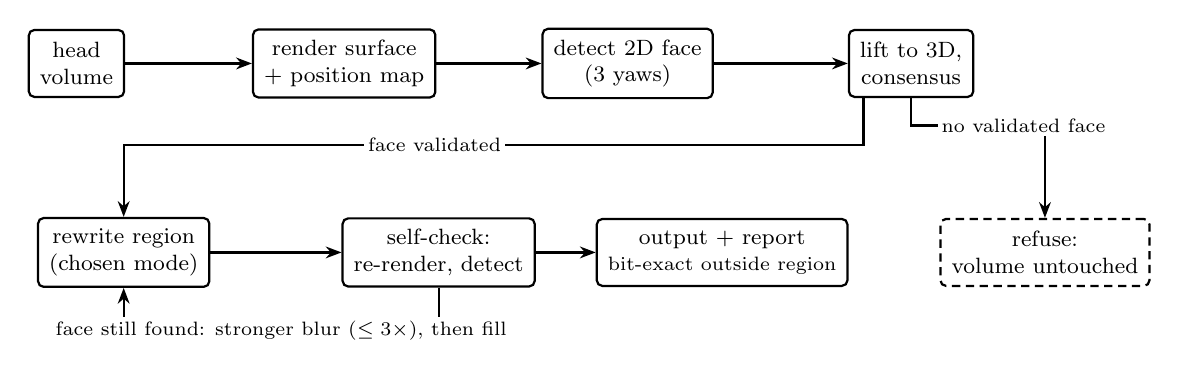
\begin{tikzpicture}[
  box/.style={draw, rounded corners=2pt, align=center, font=\footnotesize,
              inner sep=4pt, minimum height=8.5mm},
  stop/.style={box, densely dashed},
  lab/.style={font=\scriptsize, fill=white, inner sep=1.5pt},
  >={Stealth[length=2mm]}, thick]
  % row 1: find the face
  \node[box] (vol) at (0,0) {head\\volume};
  \node[box] (render) at (3.4,0) {render surface\\+ position map};
  \node[box] (detect) at (7.0,0) {detect 2D face\\(3 yaws)};
  \node[box] (cons) at (10.6,0) {lift to 3D,\\consensus};
  % row 2: rewrite and verify
  \node[box] (region) at (0.6,-2.4) {rewrite region\\(chosen mode)};
  \node[box] (check) at (4.6,-2.4) {self-check:\\re-render, detect};
  \node[box] (out) at (8.2,-2.4) {output + report\\\scriptsize bit-exact outside region};
  \node[stop] (refuse) at (12.3,-2.4) {refuse:\\volume untouched};
  \draw[->] (vol) -- (render);
  \draw[->] (render) -- (detect);
  \draw[->] (detect) -- (cons);
  \draw[->] (cons.south west) ++(0.2,0) |- ++(-1.5,-0.6) -| (region.north)
    node[lab, pos=0.25]{face validated};
  \draw[->] (cons.south) -- ++(0,-0.35) -| (refuse.north)
    node[lab, pos=0.42]{no validated face};
  \draw[->] (region) -- (check);
  \draw[->] (check) -- (out);
  \draw[->] (check.south) -- ++(0,-0.55) -| (region.south)
    node[lab, pos=0.25]{face still found: stronger blur ($\le3\times$), then fill};
\end{tikzpicture}
\caption{The pipeline. The attack is the localizer: the face is found on
surface renders, lifted to scanner space through the per-pixel position
map, and rewritten; the self-check repeats the attack on the output and
escalates until its detector stops firing, then the output is written. A
volume without a validated face is refused, never half-modified.}
\label{fig:pipeline}
\end{figure}

\paragraph{Rendering.} A CPU ray caster shades the first crossing of an
iso-surface at a fraction (0.14) of the 99th intensity percentile (for CT:
$-400$\,HU). Each $512\times512$ render also records, per pixel, where that
surface point lies in scanner space --- this is what later lifts 2D
landmarks to 3D.

\paragraph{Detection, consensus, refusal.} The embedded detector runs on
renders at yaw $-20^\circ$, $0^\circ$ and $+20^\circ$; its landmarks are
mapped to the 68-point layout and lifted to 3D through the position map.
Distances are measured in units of $d$, the detected inter-eye distance.
Views confirm each other when their lifted landmarks agree (median distance
$\le 0.45d$); a face seen in only one view must be re-found in four of seven
renders around its axis, and a six-direction sweep handles volumes stored in
a wrong orientation. A volume with no validated face is refused and left
untouched.

\paragraph{Region and modes.} The validated face fixes a region: $1.05d$ to
either side, $0.6d$ above the eyes, $0.43d$ below the chin, with a back wall
that follows the measured skin $0.07d$ ($\approx4.5$\,mm) below it. What
happens inside the region is the mode: \code{blur} applies a Gaussian
($\sigma=0.17d$); \code{adaptive}, the default, strengthens the kernel where
the image has strong edges, up to $2.5\sigma$; \code{cut} sets the region to
background; \code{block} fills it opaquely. Ears, on request, are located by
surface protrusion and cut.

\paragraph{Self-check.} The output is re-rendered from every detection yaw
at pitch $0^\circ$ and $-15^\circ$ and a $3\times3$ grid (yaw
$\{-25,0,25\}^\circ$, pitch $\{-20,0,20\}^\circ$), at the input's iso-surface,
and the same detector is run. A detection within $0.75d$ of the face counts;
blur-family modes then escalate $\sigma$ by $1.6\times$ for up to three
rounds, then fill the region opaquely. If a detection persists after the
fill, the output is still written and the residual count is reported; this
happened on \ssResidualAccepted{} of the accepted SynthStrip scans and on
\ixiResidualAccepted{} of the accepted IXI volumes. The self-check thus
optimizes the output against the very
detector that judges it; independent attackers are needed to evaluate it.

\paragraph{Brain guard; implementation.} Optionally the brain is extracted
with a pure-Rust reimplementation of SynthStrip~\cite{hoopes2022} and nothing
within 3\,mm of it is rewritten. \rv{}~\cite{radveil} is a Rust library with
a CLI, Python and C bindings and embedded detector weights; no registration,
atlas or ML framework. It is also available interactively as the
SlicerRadVeil extension~\cite{slicerradveil} for 3D
Slicer~\cite{fedorov2012slicer}, merged into the Slicer Extensions Index and
distributed with the preview (unstable) builds. To use the tool rather than
reproduce this paper, start from \code{docs/quickstart.md} in the
repository. Evaluated version: \swVersion{} (git \code{\swGit}).

\begin{figure}[tbp]
  \centering
  \fig{\linewidth}{fig_modes.png}
  \caption{One public IXI T1 scan, chosen by the script as the first IXI T1
  the adaptive run accepted without escalation. Rows, top to bottom:
  frontal surface render, $40^\circ$-yaw render, and the mid-sagittal slice
  with the anonymized region outlined in amber.
  ``Escalated'': the self-check still found a face and the region was filled.
  IXI data, CC BY-SA 3.0.}
  \label{fig:modes}
\end{figure}

% ======================================================================
\section{Evaluation}
\label{sec:eval}

\subsection{Data}
\paragraph{SynthStrip evaluation set} (v1.5, Hoopes et al.~\cite{hoopes2022};
CC BY 4.0, IXI part CC BY-SA 4.0). \ssWithImage{} full-head scans with
distributed images and manually refined brain masks (brain and CSF): IXI
T1/T2/PD/MRA/DWI (50 subjects; the IXI T1 is a spoiled gradient-echo
sequence), FSM T1 MPRAGE, T2 SPACE, PD FLASH and qT1 MP2RAGE (part of FSM was
defaced before release), ASL T1 MPRAGE and PCASL EPI, QIN 2D clinical
T1/T2/FLAIR of glioblastoma patients, and infant T1. FSM and ASL images are
stored as 8-bit integers. The \ssWithLabels{} T1 scans of IXI, FSM and ASL
carry SynthSeg/FreeSurfer label maps~\cite{billot2023}. The dataset's own
split has \ssTestCases{} test and \ssValidCases{} validation scans.

\paragraph{IXI} (CC BY-SA 3.0)~\cite{ixi}. All T1, T2 and PD volumes:
\ixiVolumes{} volumes of \ixiSubjects{} subjects from three sites (Philips
1.5\,T, Philips 3\,T, GE 1.5\,T), with age and sex. T2 and PD come from one
dual-echo acquisition; all three contrasts share the session's head pose.

\paragraph{Development overlap.} \rv{}'s defaults were measured on the
SynthStrip set and its ear model was calibrated on hand-marked pinnae of
the 50 IXI subjects in that set plus three more; these \ixiDevSubjects{}
subjects also appear in the IXI cohort. Results on the SynthStrip set are
therefore in-sample. IXI results are reported for held-out and development
subjects separately (Table~\ref{tab:ixigroups}); the held-out subjects share
sites, scanners and protocol with the development ones, so no result here is
out of distribution.

\subsection{Configurations and baselines}
\rv{} runs as \code{radveil auto --mode adaptive} with defaults unless
stated; ablations: no self-check, \code{blur}, \code{cut}, face+ears (ears
cut), brain guard, and the opt-in partial-face/auto-threshold extensions.
Baselines run in pinned x86 containers (digests in
\code{results/manifests/containers.json}; emulated on Apple silicon, so their
timings are not compared): \code{pydeface} (FSL FLIRT), \code{mri\_deface}
(FreeSurfer atlases) and Quickshear (brain mask from the original SynthStrip
container, 10\,mm buffer). On the SynthStrip set mri\_deface and Quickshear
run on every structural scan and pydeface, the slowest, on the scans \rv{}
accepted; on IXI the baselines run on a fixed random sample of 100 subjects,
on which every configuration is compared pairwise. A baseline's region is
taken to be the voxels whose stored value changed by more than half an
integer quantization step --- smaller changes are rounding from re-saving
the volume, not defacing: pydeface re-saves every voxel with up to one step
of rounding (\requantPydefaceScans{} of \requantPydefaceN{} scans), and
mri\_deface writes float32 (\dtypeMriDefaceChanged{} scans changed
datatype). This region counts
only changed voxels, whereas \rv{}'s exported region also contains voxels the
operation left unchanged; the baselines' extent is therefore, if anything,
understated.

\subsection{Quality metrics}
\paragraph{Outcome.} Accepted, refused (with the tool's reason) or error
(our infrastructure failing: a crash, a killed container; retried and never
counted as a refusal; \retriedCases{} cases needed a retry).
\paragraph{Face presence.} Whether a refusal was right is a question about
the input alone. Every SynthStrip scan, and on IXI every volume \rv{} refused
or failed on plus as many randomly drawn accepted ones, was rendered with no
tool applied (five yaws, two further iso-surface thresholds, a view from
below, mid-sagittal and mid-axial slices). The renders were shown in
shuffled order, blinded to every tool's decision, and each scan was labelled
\emph{full face} (eyes, nose, mouth and chin inside the field of view),
\emph{partial face} (e.g.\ a slab around the eyes, or a field of view ending
at the upper lip), \emph{no face} (brain-only coverage, cropped, or already
defaced) or undecidable. The labels were assigned by a vision-language model
(Claude Opus 5.5) run as blinded labellers that saw only these sheets, not
by a person; the sheets and the labelling page are released for human
relabelling. A refusal or error on a full face is a \emph{false refusal}. On
a partial face there may be too little face to fit and verify a defacing, so
a refusal is not counted as wrong; such a scan still shows part of a face
and is reported apart.
\paragraph{Visual review.} Every case leaves a QA sheet (input and output
renders, three slices with the region and expert brain mask outlined, the
attacker's on-face hits); \qaReviewed{} of \qaSheets{} sheets were reviewed by
a person in a browser page that records verdicts, and \qaFlagged{} were
flagged.
\paragraph{Integrity and extent.} Stored values outside the region,
datatype, affine and scaling; the volume of \emph{tissue} changed (input
above 10\% of its 99th percentile), since the region is mostly air.
\paragraph{Brain safety.} Anonymized voxels inside the expert mask, and the
region's closest approach to it (exact Euclidean distance transform, mm).
With SynthSeg labels, voxels in labelled brain structures (ventricles and CSF
excluded) and the distance to them. Zero counts carry a one-sided 95\%
Clopper--Pearson upper bound. Tools are compared on the \emph{paired set} of
\bsPairedN{} scans that every configuration processed; because the other
tools ran on scans \rv{} accepted, this set leans toward \rv{}'s easier
cases, and every paired comparison is conditional on acceptance. On IXI,
which has no expert masks, every tool is scored against an independent
reference, the original SynthStrip (container) on the unmodified input, on
the 100-subject sample.
\paragraph{Downstream.} The original SynthStrip on input and output: Dice of
the two brain masks and brain-volume change. On a fixed 20\% of these cases,
FSL FAST tissue segmentation (3 classes) of each skull-stripped volume:
per-class Dice and volume change. \rv{}'s Rust SynthStrip, used by its
brain check and guard, is validated against the original and the expert
masks.
\paragraph{Performance.} On an idle laptop (\hwCpu, \hwCores{} cores,
\hwMem\,GB): the CLI end to end on \profCohortN{} random accepted scans after
a warm-up run; per-stage latency in a warm process (median of 5; extra costs
as paired per-repeat differences) on \profStageN{} scans stratified by
subset; thread scaling, SIMD vs portable kernels and self-check effort
interleaved in random order; batch throughput on
\profThroughputVolumes{} distinct volumes.

\subsection{Attack suite}
\label{sec:attacks}
Table~\ref{tab:attacksummary} summarizes the four attacks. Two terms recur.
The \emph{iso-surface depth} is the rendering threshold as a multiple of the
input's: raising it moves the rendered surface inward, so a higher multiple
shows a tissue surface deeper under the skin --- at $2\times$ and beyond,
below the layer \rv{} rewrites. The \emph{release risk} is re-identification
counted over every scan a data release would contain: scans the tool refused
or failed on are counted at their clean, unmodified outcome;
\emph{accepted-only} figures, over just the processed scans, are labelled as
such.

\begin{table}[tbp]
\centering\small
\caption{The attack suite at a glance. Every attack runs on released
outputs with full knowledge of \rv{} (Section~\ref{sec:threat}).}
\label{tab:attacksummary}
\fit{\begin{tabular}{llll}
\toprule
Attack & Attacker uses & Primary metric & Results\\
\midrule
Dense detection & 2 detectors, 84 views & on-face detection rate & Table~\ref{tab:attack}\\
Face recognition & SFace + ArcFace, 4 iso-surface depths & rank-1, AUC, TAR & Tables~\ref{tab:reid}--\ref{tab:reidpaired}\\
Blur inversion & the reported kernel, Richardson--Lucy & rank-1 after inversion & Table~\ref{tab:deconv}\\
Head-shape linkage & no recognizer: radial map, rigid ICP & rank-1 linkage & Table~\ref{tab:shape}\\
\bottomrule
\end{tabular}}
\end{table}

\paragraph{Detection (a proxy).} Input and output are rendered at 7 yaws
spanning $-60^\circ$ to $+60^\circ$ $\times$ 3 pitches $\times$ 4
iso-surface depths ($0.5$--$4\times$) and attacked with the built-in
detector and YuNet~\cite{wu2023yunet}. A detection (``fire'', score
$\ge0.5$) is \emph{on-face} when its box centre lies within half an input
face width of the input's face. \emph{Core} counts fires at
$|\text{yaw}|\le20^\circ$ on the input iso-surface, inside the self-check's
own range. Wilson 95\% intervals~\cite{wilson1927} (scans of one subject
counted separately).
\paragraph{Re-identification (IXI).} Renders at yaw $-40^\circ$ to $+40^\circ$
and iso-surface depths $0.5$, $1$, $2$ and $4\times$ are embedded with
SFace~\cite{zhong2021sface} and ArcFace~\cite{deng2019arcface} (the
InsightFace w600k\_r50 weights) after 5-point alignment on YuNet landmarks;
a template is the mean over yaws. The gallery holds one clean T1 template
per subject, per depth; chance is reported per depth. Probes are the
subjects' T2 and PD scans, compared at the same depth. The \emph{fused}
attacker takes the maximum score over the four depths, for genuine and
impostor pairs alike.

Each output is aligned twice: on the face location of the unmodified input
(``oracle'') and on whatever is detected on the output itself (``blind'').
The oracle attacker uses whichever alignment scores higher; it is the
primary, strongest variant.

We report rank-1 with subject-level cluster-bootstrap 95\% intervals
(Clopper--Pearson over subjects when there are five or fewer hits), AUC,
paired clean-vs-anonymized differences with cluster-bootstrap intervals, and
a test against chance with subjects as units. The true-accept rate (TAR) at
0.1\% false accepts uses a cross-validated threshold (fitted on one half of
the subjects, applied to the other, 20 random halvings), calibrated once on
clean and once on anonymized impostors.
\paragraph{Blur inversion.} On \deconvN{} held-out subjects (one T2 each), the
anonymized region is deconvolved by Richardson--Lucy (\deconvIters{}
iterations) with the reported blur $\sigma$ and with the adaptive mode's
heavy kernel ($2.5\sigma$), then re-identified with the fused attacker.
\paragraph{Head-shape linkage (IXI).} A recognizer-free attack: the head
iso-surface is described by a radial-distance map from the vertex centroid;
candidates are ranked by robust map difference and the top 20 re-ranked by
trimmed rigid ICP of the surface points. Because IXI's contrasts share head
pose, a pose-perturbed control moves each of 150 random probes by a random
rigid motion ($10^\circ$, 10\,mm) and matches it by ICP against every
candidate, without the pose-dependent map.

% ======================================================================
\section{Results}
\label{sec:results}

\subsection{Coverage}
Table~\ref{tab:outcomes}. \rv{} accepted \ssAccepted{} of \ssCases{}
SynthStrip scans and \ssStructAccepted{} of the \ssStructCases{} structural
ones; \ssRefused{} were refused (\ssRefusedNoFace{} without a plausible face,
\ssRefusedRejected{} with candidates that failed 3D consensus,
\ssRefusedFov{} cut by the field of view) and \ssErrors{} failed. Of the
refused scans, \refusedFaceSynthstrip{} still showed a face that YuNet found
on the unmodified render. The partial-face and auto-threshold extensions
accepted \robustAccepted{} scans (\robustGained{} more, \robustGainedTouched{}
of them touching the brain mask). On IXI (Table~\ref{tab:ixi}), \ixiAccepted{}
of \ixiVolumes{} volumes were accepted (T1 \ixiAccTOnePct\%, T2
\ixiAccTTwoPct\%, PD \ixiAccPdPct\%; volumes pooled, each subject
contributing up to three); \refusedFaceIxi{} of \refusedIxi{} refused
volumes showed a detectable face.

Against the face-presence labels (Table~\ref{tab:facelabels}), \rv{}
refused or failed on \flSynthstripFalseRefusals{} of the \flSynthstripFaceN{}
SynthStrip scans with a full face (\flSynthstripFalseRefusalPct\%;
\flSynthstripFalseRefusalInfant{} of them infant scans whose surface is
buried in background noise). It accepted \flSynthstripPartialAccepted{} of
\flSynthstripPartialN{} partial faces, and of \flSynthstripNoFaceN{} scans
without a face it refused \flSynthstripCorrectRefusals{} and accepted
\flSynthstripAcceptedNoFace{}, all of them FSM scans defaced before release,
whose already-defaced region it anonymized again. On IXI, all \flIxiNotOkN{}
volumes \rv{} refused or failed on were labelled: \flIxiFalseRefusals{} had
a full face (both T1, refused as cut by the field of view) and
\flIxiNotOkPartial{} were partial faces, T2 and PD volumes whose field of
view ends between the nose and the upper lip. In fact every T2 and PD
volume in the sample, accepted or not, was a partial face. On IXI \rv{}
therefore refuses partial faces, not full ones, and the accepted shares for
T2 and PD in Table~\ref{tab:ixi} measure its acceptance of partial faces.

\begin{table}[tbp]
\centering\small
\caption{SynthStrip set, \rv{} \code{adaptive}: outcome per subset.
Filled: accepted scans whose self-check escalated to the opaque fill.
Self-check rounds: number of accepted scans with 0/1/2/3+ escalation rounds.}
\label{tab:outcomes}
\fit{\begin{tabular}{llrrrrr}
\toprule
Subset & Contrast & Scans & Accepted & Errors & Filled & Rounds 0/1/2/3+\\
\midrule
\tablebody{tab_synthstrip_outcomes}
\bottomrule
\end{tabular}}
\end{table}

\begin{table}[tbp]
\centering\small
\caption{IXI, \rv{} \code{adaptive}. Accepted: \% [Wilson 95\%; within a
row each subject contributes one volume]. Filled: accepted volumes whose
self-check escalated to the opaque fill. Brain touched: \rv{}'s own brain
check (Rust SynthStrip), with 95\% upper bound (\%); the independent
comparison is Table~\ref{tab:ixibrain}.}
\label{tab:ixi}
\fit{\begin{tabular}{llrlrrl}
\toprule
Site & Contrast & Volumes & Accepted (\%) & Errors & Filled & Brain touched\\
\midrule
\tablebody{tab_ixi}
\bottomrule
\end{tabular}}
\end{table}

\begin{table}[tbp]
\centering\small
\caption{IXI acceptance by subgroup, \% [subject-level bootstrap 95\%].
Descriptive only: sites, age and sex are confounded in IXI.}
\label{tab:ixigroups}
\begin{tabular}{lrl}
\toprule
Group & Volumes & Accepted (\%)\\
\midrule
\tablebody{tab_ixi_groups}
\bottomrule
\end{tabular}
\end{table}

\begin{table}[tbp]
\centering\small
\caption{Decisions against face presence in the input (model-assigned,
blinded labels; IXI: refused and failed volumes plus an equal random sample
of accepted ones, so IXI counts of accepted scans are of the sample, not of
the cohort). Configurations that decided identically on every labelled scan
share one row. False refusal: refused or error on a full face, \% [Wilson
95\%].}
\label{tab:facelabels}
\fit{\begin{tabular}{llrrrrlrrrrr}
\toprule
& & \multicolumn{5}{c}{Full face} & \multicolumn{2}{c}{Partial} & \multicolumn{3}{c}{No face}\\
\cmidrule(lr){3-7}\cmidrule(lr){8-9}\cmidrule(lr){10-12}
Set & Configuration & N & Acc. & Ref. & Err. & False ref.\ (\%) & N & Acc. & N & Ref.\ or err. & Acc.\\
\midrule
\tablebody{tab_face_labels}
\bottomrule
\end{tabular}}
\end{table}

\subsection{Integrity and extent}
Outside the region, stored values were unchanged in \ssBitExact{} of
\ssAccepted{} accepted SynthStrip scans and \ixiBitExact{} of \ixiAccepted{}
IXI volumes; datatype, affine and scaling were kept in \ssHeaderKept{}
(\ssScaledInputs{} inputs had non-trivial scaling, so preservation of
\code{scl\_slope} is untested here). The region had a median volume of
\ssRegionMlMedian\,ml, of which a median \ssTissueMlMedian\,ml was tissue
that changed.

\subsection{Brain safety and downstream effect}
Table~\ref{tab:brain}, Figure~\ref{fig:brain}. On all accepted SynthStrip
scans, \rv{} \code{adaptive} touched the expert brain mask in
\bsAdaptiveTouched{} of \bsAdaptiveN{} (upper bound \bsAdaptiveAllUpper\%;
median closest approach \bsAdaptiveAllMedianDist\,mm, minimum
\bsAdaptiveAllMinDist\,mm). The per-subset bounds are wide where data are few:
QIN \bsAdaptiveQinUpper\% ($n=\bsAdaptiveQinN$), infants \bsAdaptiveInfantUpper\%
($n=\bsAdaptiveInfantN$). On IXI, \rv{}'s own brain check flagged a modified
voxel inside its brain mask on \ixiBrainTouched{} of \ixiBrainChecked{}
accepted volumes (upper bound \ixiBrainTouchedUpper\%; per site and contrast
in Table~\ref{tab:ixi}). Against the independent reference
(Table~\ref{tab:ixibrain}), \rv{} touched the brain in \ixiRefAdaptiveTouched{}
of \ixiRefAdaptiveN{} volumes (upper bound \ixiRefAdaptiveUpper\%).
\rv{}'s Rust SynthStrip agreed with the
original at a median Dice of \rustDiceMedian{} (minimum \rustDiceMin,
$n=\rustN$); against the expert masks the two reached \rustExpertDice{} and
\refExpertDice. Skull-stripping the anonymized output with the original
SynthStrip gave a median Dice of \dsSsAdaptiveDiceMedian{} with the input's
mask (minimum \dsSsAdaptiveDiceMin; Table~\ref{tab:downstream}), and FAST
tissue segmentation agreed at a median grey-matter Dice of
\segAdaptiveClassDiceTwo{} ($n=\segAdaptiveN$; Table~\ref{tab:seg}).

\begin{table}[tbp]
\centering\small
\caption{Brain safety on the SynthStrip set against the expert masks, on
the paired set of scans every configuration processed (conditioned on \rv{}
accepting them; each configuration's own accepted counts are in
Tables~\ref{tab:outcomes} and~\ref{tab:facelabels}). Touched: scans with a
modified voxel inside the mask, with the one-sided 95\% upper bound (\%) and
the largest overlap (ml). Distance: closest approach, median (IQR) and
minimum (mm). Tissue: median changed tissue (ml). SynthSeg: scans with
labels, scans with a modified voxel in a labelled brain structure, median
distance to one (mm).}
\label{tab:brain}
\fit{\begin{tabular}{lrrrrlrrrrr}
\toprule
& & \multicolumn{5}{c}{Expert brain mask} & & \multicolumn{3}{c}{SynthSeg structures}\\
\cmidrule(lr){3-7}\cmidrule(lr){9-11}
Configuration & Paired & Touched & UB\% & Max ml & Distance & Min & Tissue & $n$ & Touched & Dist.\\
\midrule
\tablebody{tab_brain_safety}
\bottomrule
\end{tabular}}
\end{table}

\begin{table}[tbp]
\centering\small
\caption{IXI brain safety against an independent reference (original
SynthStrip on the unmodified input), on the 100-subject sample: volumes,
volumes with a modified voxel in the reference mask (95\% upper bound \%),
closest approach median and minimum (mm), and the largest overlap (ml).}
\label{tab:ixibrain}
\fit{\begin{tabular}{lrrrrrr}
\toprule
Configuration & Volumes & Touched & UB\% & Median & Min & Max ml\\
\midrule
\tablebody{tab_ixi_brain}
\bottomrule
\end{tabular}}
\end{table}

\begin{figure}[tbp]
  \centering
  \fig{0.82\linewidth}{fig_brain_distance.pdf}
  \caption{Closest approach of the modified region to the expert brain mask
  on the paired set, as a cumulative distribution: curves further left run
  closer to the brain, and the height of a curve at the dotted 3\,mm line
  (the brain guard's margin) is the fraction of scans that come closer than
  that. The face region is identical for \rv{}'s adaptive, blur and cut
  modes, so one curve stands for all three. The axis is cut at 40\,mm;
  mri\_deface, which rewrites voxels across the whole volume, extends
  beyond it.}
  \label{fig:brain}
\end{figure}

\begin{table}[tbp]
\centering\small
\caption{Downstream skull-stripping: the original SynthStrip on input and
output. Dice of the two masks (median, minimum) and absolute brain-volume
change (median, maximum, \%).}
\label{tab:downstream}
\fit{\begin{tabular}{llrrrrr}
\toprule
Data & Configuration & $n$ & Dice med. & Dice min & $|\Delta V|$ med. & $|\Delta V|$ max\\
\midrule
\tablebody{tab_downstream}
\bottomrule
\end{tabular}}
\end{table}

\begin{table}[tbp]
\centering\small
\caption{Downstream tissue segmentation (FSL FAST, 3 classes; for T1 class
1--3 are CSF, grey and white matter) on a fixed 20\% of the SynthStrip
downstream cases: per-class Dice median (minimum) and absolute volume change
median (maximum, \%) between input and output.}
\label{tab:seg}
\fit{\begin{tabular}{lrllllll}
\toprule
Configuration & $n$ & Dice 1 & $|\Delta V|$ 1 & Dice 2 & $|\Delta V|$ 2 & Dice 3 & $|\Delta V|$ 3\\
\midrule
\tablebody{tab_segmentation}
\bottomrule
\end{tabular}}
\end{table}

\subsection{Detection under a stronger attacker}
Table~\ref{tab:attack}. On the \atkPairedN{} paired scans the built-in
detector fired on the original face location in at least one of 84 views
on \atkAdaptiveMediapipeAnyPct\% of \rv{} \code{adaptive} outputs, and inside
its own self-check range on \atkAdaptiveMediapipeCorePct\%; YuNet on
\atkAdaptiveYunetAnyPct\% and \atkAdaptiveYunetCorePct\%. Fires inside the
self-check range arise because the probe's grid, score threshold, roll search
and on-face radius differ from the self-check's. A smoothed head keeps a
face-shaped silhouette, so detection overstates risk; identity is measured
next.

\begin{table}[tbp]
\centering\small
\caption{On-face detection on the paired SynthStrip scans where the
detector finds the input face: \% of scans [Wilson 95\%] with a fire in any
of 84 views (any) and inside the self-check range (core).}
\label{tab:attack}
\fit{\begin{tabular}{l|rll|rll}
\toprule
 & \multicolumn{3}{c|}{MediaPipe (built in)} & \multicolumn{3}{c}{YuNet (independent)}\\
Configuration & $n$ & Any & Core & $n$ & Any & Core\\
\midrule
\tablebody{tab_attack}
\bottomrule
\end{tabular}}
\end{table}

\subsection{Re-identification}
Tables~\ref{tab:reid}--\ref{tab:deconv}. The gallery held \reidArcFaceGallery{}
subjects at the skin surface (chance \reidArcFaceChance\%) and
\reidArcFaceGalleryFour{} at $4\times$; \reidArcFaceProbeScans{} T2/PD scans
were probe-able (\reidArcFaceExcluded{} excluded for lack of a detectable
clean face). Clean probes were identified at rank 1 in
\reidArcFaceControlRankFused\% of cases by the fused ArcFace attacker
(AUC \reidArcFaceControlAuc; TAR \reidArcFaceControlTar\% at 0.1\% FAR). At
the skin surface alone the clean rate was higher,
\reidArcFaceControlRankOne\%: max-fusion over depths raises impostor scores
too. We nevertheless report the fused attacker throughout, applied
identically to clean and anonymized probes. After
\rv{} \code{adaptive} the release risk was \reidArcFaceAdaptiveRisk\%
[\reidArcFaceAdaptiveRiskLo, \reidArcFaceAdaptiveRiskHi], most of it from
scans that were refused and released unmodified. On accepted scans rank-1
fell from \reidArcFaceAdaptiveAccControl\% to \reidArcFaceAdaptiveAccRank\%
[\reidArcFaceAdaptiveAccRankLo, \reidArcFaceAdaptiveAccRankHi]
($p=\reidArcFaceAdaptiveAccP$ against chance, subjects as units; rank-10
\reidArcFaceAdaptiveAccTenRank\%). With a candidate list of 84 subjects, as
in Schwarz et al.~\cite{schwarz2019}, it was
\reidArcFaceAdaptiveRankAtEightyFour\% (clean, same probes:
\reidArcFaceAdaptiveControlRankAtEightyFour\%). An attacker calibrating on
anonymized impostors accepted \reidArcFaceAdaptiveAccTarAnonCal\% of genuine
pairs at 0.1\% FAR. Depth matters (Table~\ref{tab:reiddepth}): at the skin
surface rank-1 was \reidArcFaceAdaptiveAccDepthOne\%, at $2\times$
\reidArcFaceAdaptiveAccDepthTwo\% and at $4\times$
\reidArcFaceAdaptiveAccDepthFour\% (chance \reidArcFaceAdaptiveAccDepthFourChance\%).
Without the self-check, accepted scans were identified at
\reidArcFaceAdaptiveNoverifyAccRank\%. Blind alignment gave
\reidArcFaceAdaptiveBlindRank\%; anonymized probes against an anonymized
gallery \reidArcFaceAdaptiveMatchedRank\%; the anonymized T1 against its own
original, a sanity bound, \reidArcFaceAdaptiveSameRank\%. On the paired
100-subject sample (Table~\ref{tab:reidpaired}), release-risk rank-1 was
\reidArcFacePairedPydefaceRank\% for pydeface and
\reidArcFacePairedMriDefaceRank\% for mri\_deface --- close to
\reidArcFacePairedAdaptiveRank\% for \rv{} \code{adaptive}, but for a
different reason: their outputs themselves stay recognizable (AUC
$\ge0.9$), where \rv{}'s residual risk comes mostly from refusals counted
at their clean outcome. Quickshear, which removes the whole lower face,
reached \reidArcFacePairedQuickshearRank\%. Inverting the blur with the
known kernel
(Table~\ref{tab:deconv}) did not raise rank-1 for either recognizer: ArcFace
\deconvArcFaceSigma\% and \deconvArcFaceSigmaXAdaptive\% against
\deconvArcFacePlain\% without inversion, and SFace within its interval of
the uninverted output.

\begin{table}[tbp]
\centering\small
\caption{Re-identification on IXI, fused attacker (maximum over four
iso-surfaces), oracle alignment. Accepted: probe scans the configuration
processed / probe scans it was run on. Release risk: rank-1 \% over those
scans, refused ones counted unmodified; accepted only: the processed scans.
Cluster-bootstrap 95\% intervals; AUC and TAR at 0.1\% FAR (cross-validated
threshold) on accepted scans, calibrated on clean or on anonymized impostors.
Baselines ran on a 100-subject sample; Table~\ref{tab:reidpaired} compares
all tools on it.}
\label{tab:reid}
\fit{\begin{tabular}{llllllrr}
\toprule
Recognizer & Configuration & Accepted & Release risk & Accepted only & AUC & TAR & TAR (anon.)\\
\midrule
\tablebody{tab_reid}
\bottomrule
\end{tabular}}
\end{table}

\begin{table}[tbp]
\centering\small
\caption{Re-identification of accepted \rv{} \code{adaptive} scans by
iso-surface depth, against the same probes unmodified. Gallery: subjects
with a template at that depth (chance $=1/$gallery). Rank-1 \% [95\%], AUC,
and the paired difference anonymized minus clean (percentage points,
cluster-bootstrap 95\%).}
\label{tab:reiddepth}
\fit{\begin{tabular}{llrrllll}
\toprule
Recognizer & Surface & Gallery & $n$ & Clean & Anonymized & AUC & Difference\\
\midrule
\tablebody{tab_reid_depth}
\bottomrule
\end{tabular}}
\end{table}

\begin{table}[tbp]
\centering\small
\caption{All tools on the same probes: the IXI subjects every configuration
was run on (\reidArcFacePairedProbes{} probes, \reidArcFacePairedSubjects{}
subjects). Release-risk rank-1 \% [95\%] (refused scans counted
unmodified), AUC, and the paired difference to \rv{} \code{adaptive}
(percentage points [95\%]).}
\label{tab:reidpaired}
\fit{\begin{tabular}{llrllr}
\toprule
Recognizer & Configuration & Accepted & Rank-1 & AUC & vs \rv{} adaptive\\
\midrule
\tablebody{tab_reid_paired}
\bottomrule
\end{tabular}}
\end{table}

\begin{table}[tbp]
\centering\small
\caption{Blur inversion on \deconvN{} held-out IXI T2 scans accepted by \rv{}
\code{adaptive}: fused rank-1 \% [95\%] for the clean scan, the anonymized
output, and the output deconvolved (Richardson--Lucy) with the reported
$\sigma$ and with $2.5\sigma$.}
\label{tab:deconv}
\fit{\begin{tabular}{lllll}
\toprule
Recognizer & Clean & Anonymized & Deconvolved $\sigma$ & Deconvolved $2.5\sigma$\\
\midrule
\tablebody{tab_deconv}
\bottomrule
\end{tabular}}
\end{table}

\subsection{Head-shape linkage}
Table~\ref{tab:shape}. Without any face recognizer, the head surface alone
identified clean T2/PD probes at rank 1 in \shapeControlWholeRank\% of cases
against a gallery of \shapeGallery{} (chance \shapeChance\%), and
\shapeControlOutsideRank\% using only the head outside the face sector. After
\rv{} \code{adaptive} the rates were \shapeAdaptiveWholeRank\% and
\shapeAdaptiveOutsideRank\%. With same-session pose removed by a random
rigid motion, clean probes were still identified at \shapeControlPoseSameRank\%
and anonymized ones at \shapeAdaptivePoseRank\%. On the paired sample,
\code{cut}, pydeface, mri\_deface and Quickshear gave
\shapePairedCutRank\%, \shapePairedPydefaceRank\%, \shapePairedMriDefaceRank\% and
\shapePairedQuickshearRank\% (\rv{} \shapePairedAdaptiveRank\%).

\begin{table}[tbp]
\centering\small
\caption{Head-shape linkage on IXI: rank-1 \% [95\%] and rank-10 \% against a
clean T1 shape gallery; whole head or outside the face sector; ``moved'':
probe moved by a random rigid motion before matching (no pose information).}
\label{tab:shape}
\fit{\begin{tabular}{lrlr}
\toprule
Condition & $n$ & Rank-1 & Rank-10\\
\midrule
\tablebody{tab_shape}
\bottomrule
\end{tabular}}
\end{table}

\subsection{Performance}
Table~\ref{tab:stages}, Figure~\ref{fig:scaling}. The CLI end to end took a
median \profCohortMedianS\,s per volume (90th percentile
\profCohortPNinetyS\,s, maximum \profCohortMaxS\,s) at a median peak RSS of
\profPeakRssMedian\,MB (maximum \profPeakRssMax\,MB). In a warm process the
pipeline took a median \profMedianPipelineMs\,ms; one render
\profMedianRenderMs\,ms, one detection \profMedianDetectMs\,ms; the self-check
a median \profMedianVerifyShare\% of the pipeline; the brain check
\profMedianBrainCheckS\,s more. All \profMaxThreads{} cores were
\profSpeedupMax$\times$ faster than one; SIMD kernels gave no measurable
benefit over portable ones (\profSimdSpeedup$\times$); self-check effort
fast/balanced/thorough took
\profEffortFastS, \profEffortBalancedS{} and \profEffortThoroughS\,s. Batch
processing reached \profThroughputMax{} volumes/s (\profThroughputOne{} with
one worker).

\begin{table}[tbp]
\centering\small
\caption{Per-stage latency (ms), warm process, all cores, median of 5 on
scans stratified by subset. Render and detect are per view; ``no check''
and ``full'' are the whole pipeline without and with the self-check;
``check'' and ``brain'' are paired per-repeat extra costs.}
\label{tab:stages}
\fit{\begin{tabular}{llrrrrrrrrr}
\toprule
Scan & Grid & Load & Render & Detect & Anonymize & No check & Check & Full & Brain & Save\\
\midrule
\tablebody{tab_stages}
\bottomrule
\end{tabular}}
\end{table}

\begin{figure}[tbp]
  \centering
  \fig{0.85\linewidth}{fig_scaling.pdf}
  \caption{(a) CLI speed-up with threads for one volume (median over
  scans), against the ideal linear reference. (b) Throughput of
  \code{deface\_batch} on distinct volumes.}
  \label{fig:scaling}
\end{figure}

% ======================================================================
\section{Discussion}
\label{sec:discussion}

\paragraph{What the self-check does and does not do.} It ends when one
detector stops firing at one iso-surface and a fixed set of views. Other
views, surfaces and detectors still find face-shaped surfaces, and
recognizers identify a fraction of outputs above chance, most clearly on the
iso-surface below the anonymized layer. Measured against independent
attackers, the self-check clearly reduces \emph{detection} (any-view
MediaPipe \atkAdaptiveMediapipeAnyPct\% with it against
\atkAdaptiveNoverifyMediapipeAnyPct\% without; YuNet core
\atkAdaptiveYunetCorePct\% against \atkAdaptiveNoverifyYunetCorePct\%) but
barely changes \emph{recognition}: accepted-only rank-1
\reidArcFaceAdaptiveAccRank\% with it against
\reidArcFaceAdaptiveNoverifyAccRank\% without (Tables~\ref{tab:reid}
and~\ref{tab:reidpaired}). It is not sufficient on its own. Face recognition
on renders, not detection, is the measure of residual risk, and it should be
reported for any defacer.

\paragraph{Skin depth.} \rv{} rewrites the skin and a few millimetres below
it to keep a margin from the brain. The tissue underneath still carries the
shape of the face, which a deeper render recovers (Table~\ref{tab:reiddepth}).
\code{cut} and the baselines remove that tissue; Tables~\ref{tab:brain},
\ref{tab:reidpaired} and~\ref{tab:shape} quantify the trade between residual
identity and closeness to the brain.

\paragraph{Outside the face.} Head shape links scans of one person without
any face recognizer, also after same-session pose is removed, and face-only
defacing by any tool leaves most of it (Table~\ref{tab:shape}). Whether the
link survives across sessions (repositioning, weight change, different
scanners) needs test-retest data that IXI does not have. Releasing head MRI
therefore carries a linkage risk that defacing does not address;
skull-stripped release or controlled access are the remedies.

\paragraph{Refusals.} Refusing leaves data untouched, which protects the
brain but not the person: a refused scan with a visible face is released as
is unless the pipeline around \rv{} handles it. The release-risk figures
count that. A deployment should route refused scans to a second tool and
review them.

\paragraph{Practical guidance.} For a data release we would draw these
rules from the tables. Use \code{adaptive} (the default) when the scans
should still look natural; use \code{cut} when privacy outweighs
appearance --- it removes the tissue whose shape survives blurring
(Table~\ref{tab:reiddepth}) at no extra cost in brain distance
(Table~\ref{tab:brain}). Add the brain guard when downstream morphometry
matters; it enforces a 3\,mm margin. Treat every refusal as unfinished
work: route it to a second tool or a person, because a refused scan
released as-is carries the full clean risk, which dominates the release
risk in Table~\ref{tab:reid}. Never distribute the JSON report or the
region mask. Render and look at the outputs --- the QA sheets exist for
that. And for data where linkage across releases must be impossible,
deface is the wrong tool: head shape identifies people without a face
(Table~\ref{tab:shape}), so skull-strip or use controlled access.

\paragraph{Limitations.}
\label{sec:limits}
Renders were matched to renders of other MRI contrasts from the same
session, not to photographs. Two open recognizers were used, off the shelf;
a matcher fine-tuned on renders, or a commercial one, may be stronger. Not
evaluated: generative refacing of the anonymized region, an independent
renderer, cross-session head-shape linkage, recognition at pitched views.
The SynthStrip set was used to set \rv{}'s defaults, so its results are
in-sample; the held-out IXI subjects are not out of distribution. Downstream
analysis covers skull-stripping and FAST tissue segmentation; structure
segmentation and morphometry (SynthSeg, FreeSurfer) are not evaluated.
mideface, fsl\_deface and mri\_reface were not compared. Baselines ran on a
subject sample, the independent IXI brain comparison covers only
\ixiRefAdaptiveN{} \rv{} volumes, and timing comes from one laptop. Face presence was labelled by a
vision-language model, not by radiologists; its errors would move the
false-refusal counts.

% ======================================================================
\section{Reproducibility and data}
\label{sec:repro}

The \code{paper/} directory of the repository holds the complete chain:
data download, benchmark, analysis and this manuscript. Every number,
table and figure in the PDF is a macro generated from the per-case results
in \code{results/}; none is typed by hand. Five targets cover every use:

{\footnotesize\begin{verbatim}
make -C paper env                       # Python env + radveil built from this checkout
make -C paper data DATA_DIR=/big/disk   # IXI (~13 GB), SynthStrip (~7 GB), models, containers
make -C paper smoke DATA_DIR=/big/disk  # a few cases through every stage (~10 min)
make -C paper all   DATA_DIR=/big/disk  # every run, analysis and the PDF (~12 h on a laptop)
make -C paper pdf-only                  # this PDF from committed results (no data, no Rust)
\end{verbatim}}

\noindent Three mechanisms keep a rerun honest: every image, mask and label
map is checksummed against a committed manifest before any run; each case is
recorded as one JSON line carrying the code revision, and the benchmark
refuses to mix revisions; runs are resumable, so a crash never silently
drops cases. Face embeddings and
head-shape descriptors are biometric templates of dataset participants: they
are computed locally and not distributed, so the re-identification and
shape numbers can be recomputed only with the data; their committed
summaries are what the document uses.

\paragraph{Licences.} IXI: CC BY-SA 3.0; SynthStrip set: CC BY 4.0 (IXI
part CC BY-SA 4.0); results derived from IXI are shared under CC BY-SA 4.0.
YuNet: MIT; SFace: Apache-2.0; ArcFace weights (InsightFace buffalo\_l):
non-commercial research use only; FSL (FAST, FLIRT): free for non-commercial
use. \rv: Apache-2.0.

\clearpage  % flush remaining floats before the references
\bibliographystyle{unsrtnat}
\bibliography{refs}

\end{document}
